% TEMPLATE for Usenix papers, specifically to meet requirements of
%  USENIX '05
% originally a template for producing IEEE-format articles using LaTeX.
%   written by Matthew Ward, CS Department, Worcester Polytechnic Institute.
% adapted by David Beazley for his excellent SWIG paper in Proceedings,
%   Tcl 96
% turned into a smartass generic template by De Clarke, with thanks to
%   both the above pioneers
% use at your own risk.  Complaints to /dev/null.
% make it two column with no page numbering, default is 10 point

% Munged by Fred Douglis <douglis@research.att.com> 10/97 to separate
% the .sty file from the LaTeX source template, so that people can
% more easily include the .sty file into an existing document.  Also
% changed to more closely follow the style guidelines as represented
% by the Word sample file. 

% Note that since 2010, USENIX does not require endnotes. If you want
% foot of page notes, don't include the endnotes package in the 
% usepackage command, below.

% This version uses the latex2e styles, not the very ancient 2.09 stuff.
\documentclass[letterpaper,twocolumn,10pt]{article}
\usepackage{usenix,epsfig,endnotes}
\usepackage{graphicx}
\usepackage{url}
\usepackage{listings}
\usepackage{subfigure}
\usepackage{paralist}
\usepackage{textcomp}
\usepackage{xspace}
\usepackage{ifthen}
\usepackage{amsmath}
\usepackage{amssymb}
\usepackage{color}
\usepackage{algpseudocode}
\usepackage{algorithm}

\newcommand{\yixin}[1]{\emph{\color{red}(#1)}}
\newcommand{\annie}[1]{\emph{\color{blue}(#1)}}


\newcommand{\comment}[1]{}

\begin{document}

%don't want date printed
\date{}

%make title bold and 14 pt font (Latex default is non-bold, 16 pt)
\title{\Large \bf Countermeasures Against Active Routing Attacks on Tor}
\author{Yes, we need a more exciting title. Maybe giving it a nice name?}

%for single author (just remove % characters)
%\author{
%{}\\
%Princeton University
%\and
%{}\\
%Princeton University
%\and
%{}\\
%Princeton University
% copy the following lines to add more authors
% \and
% {\rm Name}\\
%Name Institution
%} % end author

\maketitle

% Use the following at camera-ready time to suppress page numbers.
% Comment it out when you first submit the paper for review.
\thispagestyle{empty}

\subsection*{Abstract}
Anonymity systems such as Tor are known to be vulnerable to network-level adversaries who can observe both ends of the communications to deanonymize Tor users. Recent works have shown that Tor is susceptible to the previously unknown active BGP routing attacks, which expose Tor users to more potential network-level adversaries. This paper aims at mitigating such active routing attacks against Tor. We first present a new measurement study on the resilience of the Tor network to active BGP prefix attacks. We show that Autonomous Systems which carry a large portion of Tor traffic, such as OVH, only have relatively low resilience to active attacks. Next, we present a novel guard relay selection algorithm which incorporates resilience of relays into considerations. We show that the new algorithm successfully lowers the probability of a Tor client being affected by an attack by 35\%, and at the same time provides better anonymity to the Tor client. Finally, the paper demonstrates a live monitoring framework that can detect routing anomaly on the Tor network in real time. 

%We also present a set of novel countermeasures that will help 
%prevent these types of attacks from being successful: a new path selection algorithm, 
%a live monitoring framework that uses a variety of heuristics for attack detection, and 
%suggestions for Tor relay operators. 

\section{Introduction}

The Tor network ~\cite{dingledine2004tor} has been the most widely used system for anonymous communications that protect user identity from untrusted parties who have access to user traffic. Tor serves millions of users and carries terabytes of traffic everyday with its network of over 7,000 relays ~\cite{tormetrics}, which makes it a popular target for adversaries who wish to break the anonymity of the users. 

Tor is known to be vulnerable to traffic correlation attacks. An adversary who can observe the traffic at both ends of the communication (i.e., between Tor client and entry relay, and between exit relay and the destination server) can perform  correlation analysis on packet sizes and timings to deanonymize the Tor users ~\cite{shmatikov2006timing} \cite{syverson2001towards}. Network-level adversaries, i.e., autonomous systems (ASes), that lie on the path between Tor client and entry relay, and between exit relay and the destination server have been shown to be at such a compromising position to deanonymize Tor clients ~\cite{feamster2004location}, \cite{edman2009awareness}, \cite{johnson2013users}. More recently, researchers have further exploited the dynamics of BGP routing that exaggerated this threat by enabling more network-level adversaries to be at the compromising position \cite{sun2015raptor}, including active BGP prefix attacks which were not being studied previously on Tor. 

Building countermeasures to defend Tor against such malicious AS-level adversaries is an urgent challenge facing the research community. Past works have explored AS-aware relay selection algorithms that minimize the chance of selecting Tor relays with the same AS lying on both ends of the communication paths ~\cite{edman2009awareness}, \cite{akhoondi2012lastor}, \cite{starov2015measuring}. However, all these work only focus on mitigating \emph{passive} attacks in which AS-level adversaries only passively observe traffic instead of launching any \emph{active} attacks. It has been shown that active BGP routing attacks can pose new threats on Tor users and there were Tor relays that already got affected in past real-world BGP attacks \cite{sun2015raptor}. Thus, these motivated our work on developing countermeasures against such active BGP attacks on Tor which have been previously understudied. 

In this paper, our contributions consist of three parts. First, we quantify the vulnerability of the current Tor network to active BGP prefix hijacks and interceptions. Second, we develop proactive approaches to lower the probability of being affected by such attacks, which includes a novel Tor guard relay selection algorithm. Finally, we present a live monitoring framework on Tor that can detect routing anomalies in Tor relays. 
\\
\textbf{Measurement on the Tor network.} We measure the vulnerability of the current Tor network by calculating the resilience to BGP prefix attacks for all ASes that contain Tor relays. Based on the current internet topology ~\cite{topology} and Tor consensus data ~\cite{torconsensus}, we first leverage an AS-resilience metric ~\cite{lad2007understanding} to measure resilience to \emph{all} possible hijacking scenarios. Then, we further extend the metric to analyze interception attack scenarios and measure resilience to interception attacks launched by Tier 1 ASes. Finally, we perform a case study on the state of Tor resilience during a past known attack - the Indosat hijack in 2014. Our keys findings are:
\begin{itemize}
\item Resilience values corresponding to hijack attacks for all Tor-related ASes are similar to a normal distribution, where most ASes fall in the middle of the spectrum. However, some ASes which are responsible for high number of relays and/or high bandwidths have low resilience values, i.e., AS 16276 (OVH) which contains 339 Tor relays only has resilience value of 0.32 on a scale of $[0,1]$.
\item Resilience values corresponding to interception attacks for all Tor-related ASes are skewed towards higher resilience. However, similar to that in hijack resilience, some ASes (i.e., OVH) carrying high bandwidths have relatively low resilience. 
\item Average Tor AS resilience has increased each year from 2008 to 2016. 
\item 73\% of the Tor-related ASes that were affected in Indosat hijack in 2014 had resiliency values $< 0.6$.
\end{itemize}
\textbf{Proactive approaches.} First, we start a campaign by contacting Tor relay operators to move their relays into a more specific prefix range, i.e., /24. We have successfully cooperated with Princeton University to move a Tor relay into a /24 prefix from the original /16 prefix. We also show that the increase in routing table size due to announcing /24 prefixes for Tor relays is negligible. Second, we propose and implement a novel Tor guard relay selection algorithm which incorporates AS resilience of the relays into considerations. Our guard relay selection algorithm is first algorithm to consider resilience to active BGP routing attacks on Tor ~\cite{sun2015raptor}. The algorithm combines resilience and bandwidth into relay selection to ensure security as well as performance. Our evaluation shows that the algorithm achieves 35\% reduction in probability of being affected by a prefix hijack attack and 49\% improvement on sender anonymity bound compared to the current Tor relay selection algorithm. At the same time, it does not suffer any performance loss based on a real world evaluation on page load time from Alexa Top 100 sites. 
\\
\textbf{Reactive approaches.} We build a live monitoring framework that monitors routing activities on Tor relays in real time. The monitoring framework consists of two parts: BGP monitoring framework which monitors the control plane, and Traceroute monitoring framework which monitors the data plane. BGP monitoring framework collects live BGP announcement data from BGP Stream ~\cite{bgpstream}, in combination with latest hourly Tor relay data, and detects any routing anomaly in real time. Traceroute monitoring framework utilizes Planetlab nodes to actively send traceroute requests to a selective set of Tor relays (i.e., high bandwidth relays) to monitor routing anomaly in the data plane. We believe our live monitoring framework will help enhance the transparency of the Tor network against active BGP attacks.
\\
The paper is organized as follows. Section 2 provides a brief overview of background and related work on Tor.  Section 3 describes the metrics and methodology used to measure Tor relay resilience to active BGP prefix hijack and interception attacks. Section 4 discusses our campaign on moving Tor relays to /24 prefixes and presents our new Tor guard relay selection algorithm. Section 5 demonstrates our design for the live monitoring framework and describes deployment experiences. Section 6 discusses potential obstacles and shortcomings of the current approaches and directions for future work. Finally, we conclude in Section 7. 
%Recently, researchers have shown that AS-level adversaries can exploit the dynamics of BGP routing and launch new attacks on Tor \cite{sun2015raptor}, including both passive attacks exploiting routing asymmetry and natural churn, as well as active attacks with BGP prefix hijacking/interception. Thus, these new attacks urge the need to build countermeasures to defend Tor against such malicious AS-level adversaries. In this work, we will focus on developing countermeasures against active BGP routing attacks. 
%
%There are two potential ways to counter the attacks: (1) Mitigating traffic interception, and (2) Mitigating correlation attacks. However, mitigating correlation attacks usually involve employing extra encryption schemes and/or packet obfuscation, which either requires extensive engineering efforts, or could result in high latency of Tor. Thus, given the constraints of mitigating correlation attacks, we will build countermeasures that focus on mitigating traffic interception, more specifically, against active BGP routing attacks. Our approach includes two parts, as following. 
%
%The first part is a set of proactive approaches to countering BGP attacks.  These approaches make it more difficult for an attacker to hijack Tor traffic.  There's a surprisingly large number of Tor relays that are announced in prefixes that are larger than /24, which means they are vulnerable to sub-prefix hijack attacks.  Therefore, one countermeasure is for operators to announce Tor relays in a /24.  Similarly, operators can use a static route to guard relays, so that the traffic cannot be hijacked.  In the case of equal-length prefix hijack attacks, we also propose a new path selection algorithm for the path from the client to the guard relay.  
%
%The second part is a reactive approach: a monitoring framework that can detect attacks in real-time.  We have built a BGP monitoring framework for the Tor network that uses multiple different techniques to detect suspicious prefix announcements.  This is used in conjunction with a traceroute monitoring framework for validation of path changes and suspicious paths.  
%
%Previous work has shown that the Tor network is susceptible to AS-level adversaries, and specifically prefix hijacks.  In this work, we measure how resilient each AS -- with at least one Tor relay -- is to a prefix hijack from anywhere else on the Internet.  Our contributions are:

%\begin{itemize}
%\item Measure hijack resiliency of the ASes that contain relays and compare the resiliency of ASes that contain more relays to those that contain few relays.
%\item Measure interception resiliency of the ASes that contain relays and compare the resiliency of ASes that contain more relays to those that contain few relays.
%\item Quantify how much resiliency to hijacks and interceptions on the Tor network differs year to year, starting in 2008.
%%\item Quantify if Tor relays have become more resilient since the initial network was built.
%%\item Quantify how fast relay resilience changes.
%\item Build a real-time monitoring system for the Tor network, which uses both the control plane and data plane.
%\item Develop a new guard selection technique for Tor clients, which we evaluate and show is more resistent to hijack attacks.
%\item Discuss experiences with relay operators in regards to announcing relays in a /24.
%\end{itemize}



\section{Background and Related Work}
Here we discuss network level adversaries on the Tor network and past work on defending against such network level adversaries. 

\subsection{Network Adversaries on Tor}
%To communicate with a destination, Tor clients establish
%layered circuits through three subsequent Tor relays. The
%three relays are referred to as: entry (or guard) for the
%first one, middle for the second one, and exit relay for
%the last one. To load balance its traffic, Tor clients select
%relays with a probability that is proportional to their
%network capacity. Encryption is used to ensure that each
%relay learns the identity of only the previous hop and the
%next hop in the communications, and no single relay can
%link the client to the destination server.
%
%It is well known that if an attacker can observe the
%traffic from the destination server to the exit relay as well
%as from the entry relay to the client (or traffic from the
%client to the entry relay and from the exit relay to the
%destination server), then it can leverage correlation between
%packet timing and sizes to infer the network identities
%of clients and servers (end-to-end timing analysis).
%This timing analysis works even if the communication is
%encrypted~\cite{sun2015raptor}.
%Network-level adversaries are known in anonymity networks. 
Feamster and Dingledine \cite{feamster2004location} first investigated AS-level adversaries in anonymity networks, and they showed that some ASes could appear on nearly 30\% of entry-exit pairs. Murdoch and Zielinski \cite{murdoch2007sampled} later demonstrated the threat posed by network-level adversaries who can deanonymize users by performing traffic analysis. Furthermore, Edman and Syverson \cite{edman2009awareness} demonstrated that even given the explosive growth of Tor during the past years, still about 18\% of Tor circuits result in a single AS being able to observe both ends of the communication path. In 2013, Johnson \emph{et al.} \cite{johnson2013users} evaluated the security of Tor users over a period of time, and the results indicated that a network-level adversary with just a low-bandwidth cost could deanonymize any user within three months with over 50\% probability and within six months with over 80\% probability.

While all prior research, to our knowledge, focus on passive adversaries, more recently, Sun \emph{et al.} ~\cite{sun2015raptor} discovered the threat posed by active AS-level adversaries, who can perform active BGP routing attacks to put themselves onto the path between client-entry and/or exit-destination, and thus be able to observe Tor traffic. The paper also showed from past BGP data that during past known real-world BGP prefix attacks, Tor relays were affected as well - i.e., in the Indosat hijack in 2014, among the victim prefixes there were 44 Tor relays, and 33 of them were guard relays which had direct connections with Tor clients. 

\subsection{Tor Path Selection against Network Adversaries}
The existence of network-level adversaries motivates the research on AS-awareness in path selection in Tor. In 2012, Akhoondi \emph{et al.} \cite{akhoondi2012lastor} proposed LASTor, a Tor client which takes into account AS-level path and relay locations in selecting a path; although our work differs by considering relays' resilience to active attacks and relays' capacity. Recently, Nithyanand \emph{et al.} \cite{starov2015measuring} constructed a new Tor client, Astoria, which adopted a new path selection algorithm that considered more aspects - relay capacity, asymmetric routing, and colluding ASes. However, Astoria only considers a passive AS-level attacker and does not consider the case of active routing attacks.\\
\\
This motivates our work on defending Tor against active AS-level adversaries who can launch active routing attacks such as BGP prefix hijacks and interceptions. Towards this goal, it is important to understand AS-level Internet topology and network path predictions. Lad \emph{et al.} \cite{lad2007understanding} investigated the relationship between Internet topology and prefix hijacking, and provided a metric for evaluating AS resilience to active prefix hijack attacks. Although the study was conducted in 2007 when there were far less ASes than now, and the study only simulated a partial attack scenario of 1000 randomly selected ASes as attackers, it provides a foundational starting point for our work. Thus, in section ~\ref{hijack_interception_measurement}, we will start with applying the AS resilience metric to the Tor network, but considering \emph{all} attack scenarios; then, we will further extend the metric to evaluate AS resilience to active prefix \emph{interception} attacks, a novel metric and measurement. In Section ~\ref{subsec:relayselection}, we incorporate the AS resilience metric into the Tor guard relay selection algorithm. 


%RAPTOR attacks are a suite of attacks that can be launched by 
%Autonomous Systems (ASes) to compromise user anonymity.  There are 
%three different types of attacks in this classification.
%
%{\bf Asymmetric Traffic Analysis.} AS-level adversaries can
%exploit the asymmetric nature of Internet routing to increase
%the chance of observing at least one direction of
%user traffic at both ends of the communication.
%
%{\bf Natural Churn.} AS-level adversaries can exploit natural churn in Internet
%routing to lie on the BGP paths for more users over
%time.
%
%{\bf BGP Hijacks.} Strategic AS-level adversaries can manipulate Internet
%routing via BGP hijacks (to discover the users using
%specific Tor guard nodes) and interceptions (to perform
%traffic analysis).

\section{Measuring Tor's Current State of Resiliency to Hijack Attacks}

Because the Tor network is susceptible to network-level adversaries, we aim to quantify how much of the Tor network would be affected by a BGP prefix hijack.  First, we look at how to evaluate the Tor network in terms to susceptibility to hijack attacks.  The metric used helps enlighten the community about the state of the Tor network, in terms of how resilient the relays are to hijack attacks.  Next, we modify the metric to quantify how resilient the Tor network is to prefix interception attacks by Tier 1 ASes.  This helps quantify how vulnerable the Tor network is to network-level adversaries in a novel way.  Specifically, we measure:

\begin{itemize}
\item Resiliency (to prefix hijack attacks) of the ASes that contain relays and compare the resiliency of ASes that contain more relays to those that contain few relays.
\item Resiliency (to prefix interception attacks) of the ASes that contain relays and compare the resiliency of ASes that contain more relays to those that contain few relays.
\item How much resiliency to hijacks and interceptions on the Tor network differs year to year, starting in 2008.
\end{itemize}

\subsection{Hijack Resilience Methodology}
\label{hijack_methodology}

Previous work has tackled questions of AS resilience using simulations of the entire Internet \cite{lad2007understanding}.  We build off of this work by applying these metrics to the Tor network.  \cite{lad2007understanding} explains the probability of a node $v$ being deceived by a given false origin $a$ announcing a route that belongs to true origin $t$:

\begin{equation}
\bar{\beta}(t,a,v) = \frac {p(v,t)} {p(v,t) + p(v,a)}
\end{equation}

where $p(v,a)$ is the number of equally preferred paths from node $v$ to false origin $a$ and $p(v,t)$ is the number of equally preferred paths from node $v$ to true origin $t$.  Using this probability, the same researchers introduced the resiliency metric -- the resilience of a node $t$ is the fraction of nodes that believe the true origin $t$ given an arbitrary  hijack against $t$:

\begin{equation}
R(t) = \sum_{a \in N} \sum_{v \in N} \frac {\bar{\beta}(t,a,v)} {(N-1)(N-2)}
\end{equation}

where N is the total number of ASes.

In order to measure the resiliency of Tor-relates ASes, we first use an Internet topology~\cite{caida} to get all of the AS relationships, and construct and AS-level graph.  We identify the Tor-related ASes and simulate prefix hijacks on the graph. Specifically, our methodology consists of:

\begin{enumerate}
\item Construct an AS-level graph from an Internet topology.
\item Identify ASes that have at least one Tor relay.
\item Calculate the number of equally preferred paths from AS A to AS B, where AS B is a Tor-related AS.
\item Calculate the number of equally preferred paths from AS A to AS C, where AS C is the attacking (hijacking) AS.
\item Calculate resiliency using Equation (2).
\end{enumerate}

We follow this methodology for every AS A $\neq$ a Tor-related AS, every AS C $\neq$ a Tor-related AS, and for every AS B $=$ Tor-related AS.  Algorithm~\ref{algo:calcres} shows the steps we take on the AS graph to calculate the resiliency.

\begin{algorithm}
\caption{Algorithm to calculate prefix hijack resiliency.}
\label{algo:calcres}
\begin{algorithmic}
\Function{CalcResilience}{graph $G$, node $t$}
    \State \Call{CalcPathsFromNode}{$G,t$}
    \State $zeros(R)$
    \For{each reachable node $v$ from node $t$} 
    	\If{node $v$ contains Tor guard/exit relays}
		\State $n \gets $ num. of less preferred nodes than node $v$
		\State $R[v] \gets n + \bar{\beta}(v,a,t)$ $\forall$ equally preferred node a
	\EndIf
    \EndFor
    \State \Return $R$
\EndFunction
\end{algorithmic}
\end{algorithm}

Note that, the $\Call{CalcPathsFromNode}{G,t}$ step above requires AS-level path predictions. Previous works have shown that AS level paths are determined mainly based on two preferences~\cite{starov2015measuring}:

\begin{itemize}
\item Local Preference
\item Shortest Path
\end{itemize}

Further more, the AS paths should also have the \emph{valley free} property. Thus, we use breadth first search to traverse the graph from a given source node based on this property and the preferences. We first explore provider-customer paths, which are the most preferred; next, we explore one peer-to-peer path followed by a sequence of provider-customer paths, which are the next preferred; finally, we explore customer-provider paths followed by an optional peer-to-peer path and then followed by a sequence of provider-customer paths. Note that, nodes are explored in the most preferred to least preferred order, and those which are explored in the same step are equally preferred. This ordering will help the above resiliency calculation. 

%There is also space for metrics regarding specific relays' resiliency to BGP prefix hijack attacks, as well as metrics regarding BGP prefix interception attacks (AS- and relay-level).  

%  We also plan to specifically look at the resiliency of guard relays (as a group) as well as exit relays (as a group). 

\subsection{Interception Resiliency Methodology}
Next we measure the resiliency of Tor-related ASes to prefix interception attacks.  We modify the methodology from Section~\ref{hijack_methodology} in the following way:

\begin{enumerate}
\item Construct an AS-level graph from an Internet topology.
\item Identify ASes that have at least one Tor relay.
\item Calculate the number of equally preferred paths from AS A to AS B, where AS A $\neq$ AS B, AS A and AS B are not Tor-related ASes, and there must be a Tor relay on the path from AS A to AS B.
\item Calculate the number of equally preferred paths from AS A to AS B, where AS A $\neq$ AS B, AS A and AS B are not Tor-related ASes, there must an AS C (intercepting AS) on the path from AS A to AS B, and no Tor-related AS on the path from AS A to AS B.
\item Calculate resiliency using the equation described above.
\end{enumerate}

\subsection{Current Hijack Resiliency Results}

We obtained the list of Tor guard/exit relays from Tor consensus in December 2015 and retrieved their belonging ASes. Then, we downloaded the AS topology published by CAIDA in December 2015. We evaluated the resiliency of each of the ASes which contain Tor guard/exit relays based on the AS topology using the method in ~\cite{lad2007understanding}. 

The AS topology contains 52680 ASes, in which 612 ASes contain a total of 2548 Tor guard/exit relays. We simulated \emph{all} possible hijacking scenarios against each of the 612 ASes, totaling $52679 \times 612 = 32,239,548$ prefix hijacks. Thus, we first calculate the resiliency of each Tor AS from each of the 52680 ASes as the \emph{source} AS as following, and then sum up the resulting resiliency $R$ to obtain the total resiliency for each of the Tor ASes. 

After calculating the hijack resilience for each AS that contains at least one Tor relay, we can see that most ASes lie in the middle of the spectrum for resilience (as shown in Figure~\ref{fig:resilience_histogram}).

\begin{figure}
\centering
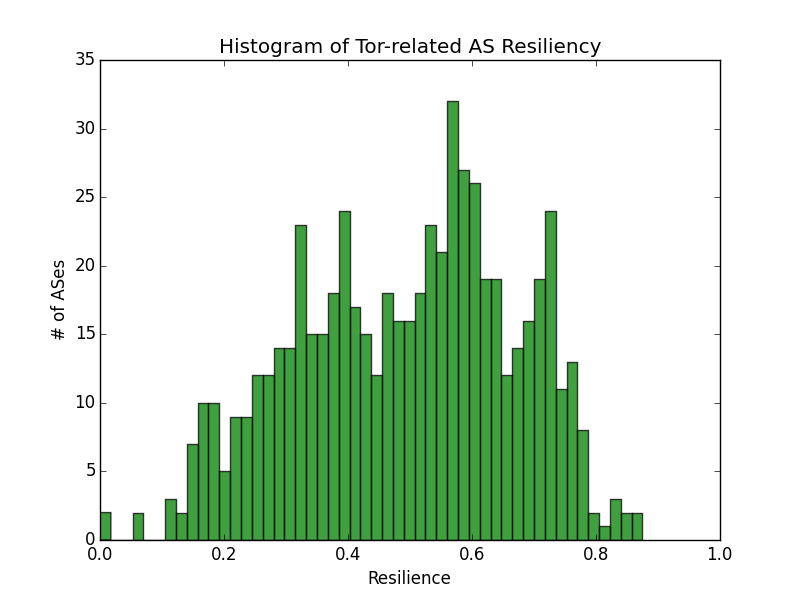
\includegraphics[width=.5\textwidth]{resilience_histogram}
\caption{A histogram of resilience values for all ASes that contain a Tor relay.}
\label{fig:resilience_histogram}
\end{figure}

We also measured the resilience to interception attacks for each Tor-related AS.  The distribution of interception resilience values is shown in Figure~\ref{fig:interception_histogram}, and we can see that many Tor-related ASes have a much higher resiliency to interception attacks that could be carried out by Tier 1 ASes.  

\begin{figure}
\centering
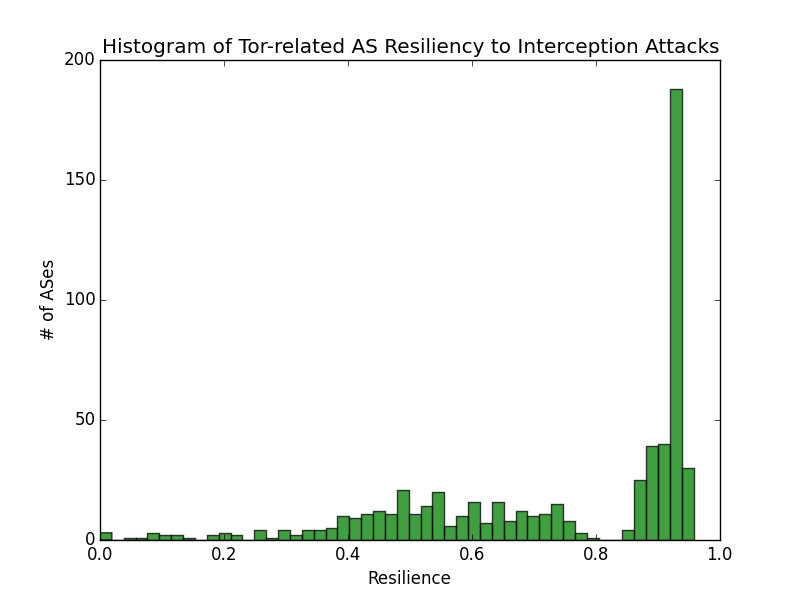
\includegraphics[width=.5\textwidth]{interception_resiliency}
\caption{A histogram of resilience values for all ASes that contain a Tor relay in 2015.}
\label{fig:interception_histogram}
\end{figure}

We then looked at which ASes had the most relays, and what their corresponding resilience is; ideally, ASes with more relays are also more resilient to hijack attacks.  Figure~\ref{fig:res_relays} shows the resilience value for an AS and the AS's corresponding number of relays.  

\begin{figure}
\centering
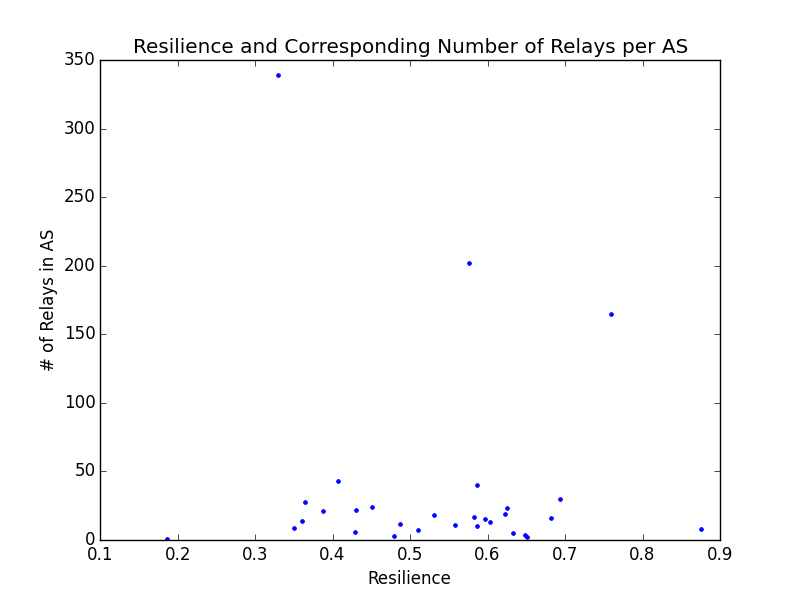
\includegraphics[width=.5\textwidth]{res_num_relays}
\caption{Resilience values for each AS and each AS's corresponding number of relays.}
\label{fig:res_relays}
\end{figure}

We can see one outlier - AS16276 - which contains 339 relays; unfortunately, this AS also has a relatively low resilience against hijack attacks.  This motivates our proactive and reactive countermeasures against hijack attacks.

\begin{figure}
\centering
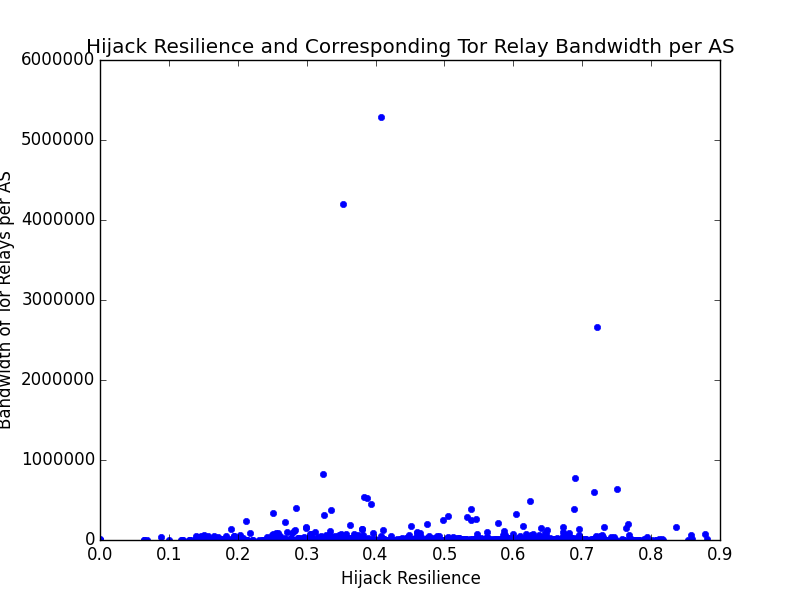
\includegraphics[width=.5\textwidth]{hijack_bandwidth}
\caption{Bandwidth of all Tor relays in an AS, and the corresponding AS hijack resiliency.}
\label{fig:hijack_bw}
\end{figure}

\begin{figure}
\centering
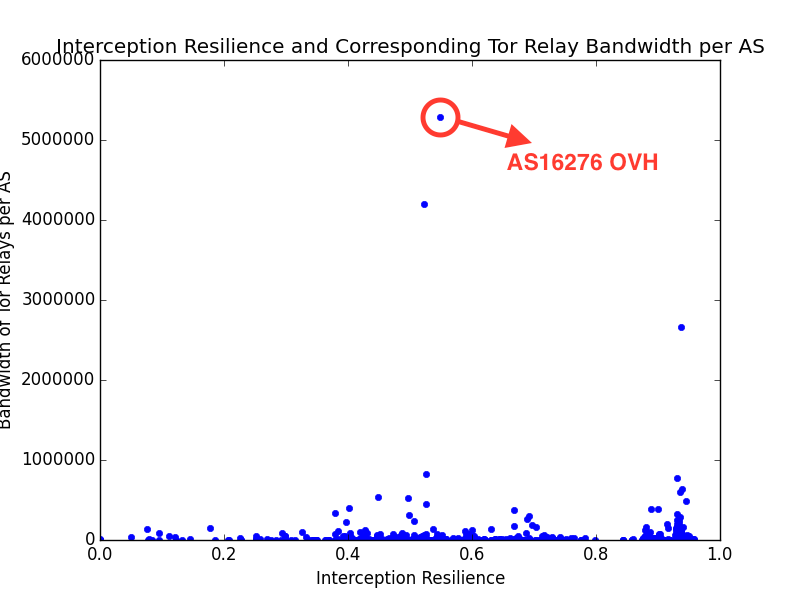
\includegraphics[width=.5\textwidth]{interception_bandwidth}
\caption{Bandwidth of all Tor relays in an AS, and the corresponding AS interception resiliency.}
\label{fig:interception_bw}
\end{figure}

\subsection{Longitudinal Resiliency Results}

We conducted our measurements on past data to analyze the hijack resiliency trend on the Tor network.  Figure~\ref{fig:resilience_trend} shows the average AS resiliency to hijack attacks each year.  We can see that the average resiliency has increased since 2008, but still remains below .50.  

\begin{figure}
\centering
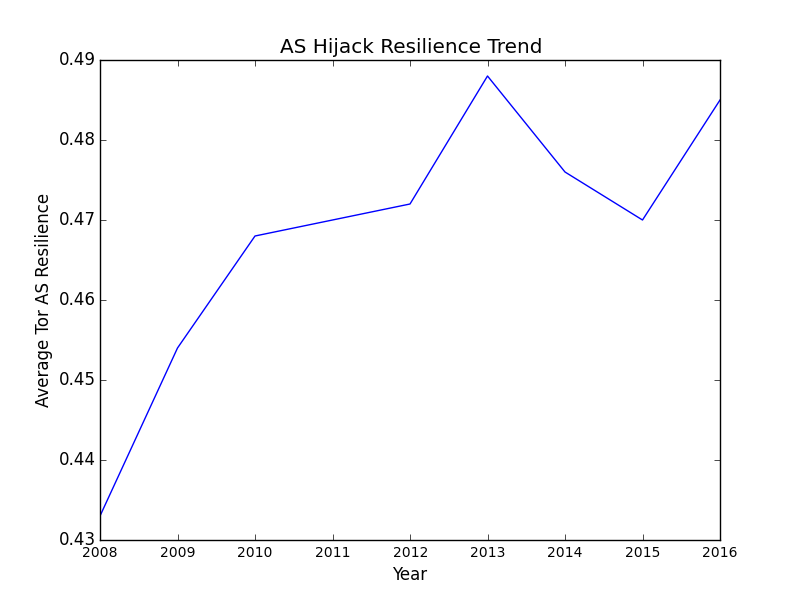
\includegraphics[width=.5\textwidth]{hijack_resilience_trend}
\caption{Average Tor AS resilience each year from 2008-2016.}
\label{fig:resilience_trend}
\end{figure}

\subsection{Case Study: Indosat 2014}
In 2014, Indosat, one of Indonesia's largest telecommunications networks, announced 417,038 new prefixes, but it usually only announces about 300 prefixes~\cite{indosat2014}.  In previous work, we found that this compromised 44 Tor relays, 38 of which were guard relays and 17 of which were exit relays (11 hijacked relays were both guards and exits)~\cite{sun2015raptor}.  We calculated the hijack resilience of the hijacked ASes; the results are shown in Figure~\ref{fig:case_study}.  We can see that the AS hijack resiliency ranges from 0.0 to .76, with most ASes falling in the middle of the spectrum. This means that even ASes with relatively high resilience values (.72 and .76) have the potential to be hijacked.  

\begin{figure}
\centering
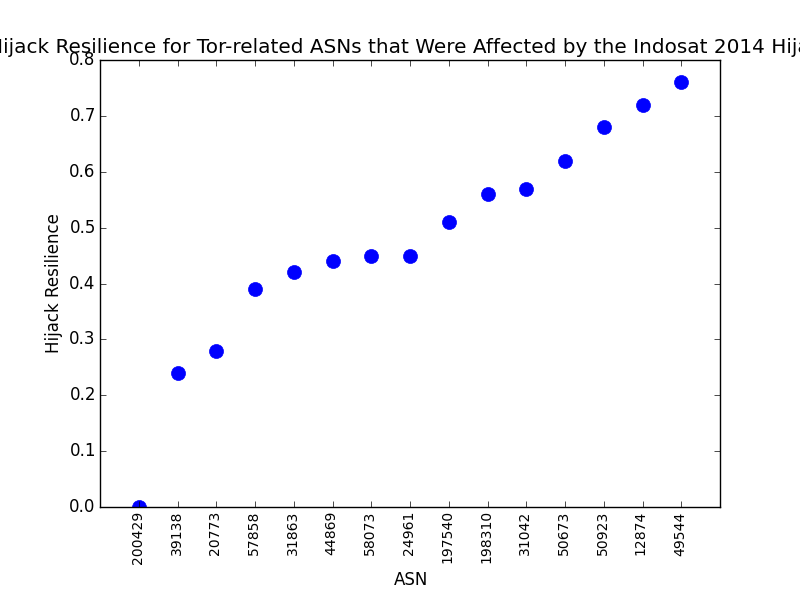
\includegraphics[width=.5\textwidth]{case_study_graph}
\caption{The ASes that contain at least one Tor relay, and were affected by the Indosat hijack attack in 2014, along with their corresponding hijack resiliency values.}
\label{fig:case_study}
\end{figure}

\section{Proactive Approaches}
\label{sec:proactive}
Sun \emph{et al.} \cite{sun2015raptor} recently demonstrated a successful real-world BGP routing attack on a Tor guard relay by announcing a more-specific prefix (i.e., /24 prefix against /23 prefix), which covers the guard relay. We have shown in Section \ref{hijack_interception_measurement} that network-level adversaries can hijack a portion of the traffic by announcing an equally-specific prefix (i.e., same prefix length). To counter these two routing attacks, we propose two methods, respectively: 1) convincing relay operators to move the relay into a /24 prefix to defend against a more-specific prefix attack, and 2) introducing a new Tor guard relay selection algorithm that minimizes the likelihood that a Tor client sees a hijacked route in the case of an equally-specific prefix attack.

\subsection{Using /24 Prefixes}
\label{subsec:24prefix}
Network-level adversaries can hijack internet traffic by announcing a more-specific prefix that belongs to the true origin AS. Since BGP routing prefers longer prefixes over shorter ones, the traffic will go to the false origin with the more-specific prefix instead. The longest prefix length that BGP usually accepts is /24, and thus any prefix that's shorter than /24 is vulnerable to more-specific prefix attacks. Sun \emph{et al.} \cite{sun2015raptor} recently found that more than 90\% of BGP prefixes hosting relays are
shorter than /24, making them vulnerable to a more-specific BGP prefix attack. 

%We measured the distribution of prefix lengths in relation to Tor bandwidth using the Tor consensus data in January 2016; this is shown in ~\ref{fig_prefixlen}. Consistent with the findings in \cite{sun2015raptor}, a large percentage of the bandwidth are under prefixes shorter than /24. 

%\begin{figure}[ht!]
%\centering
%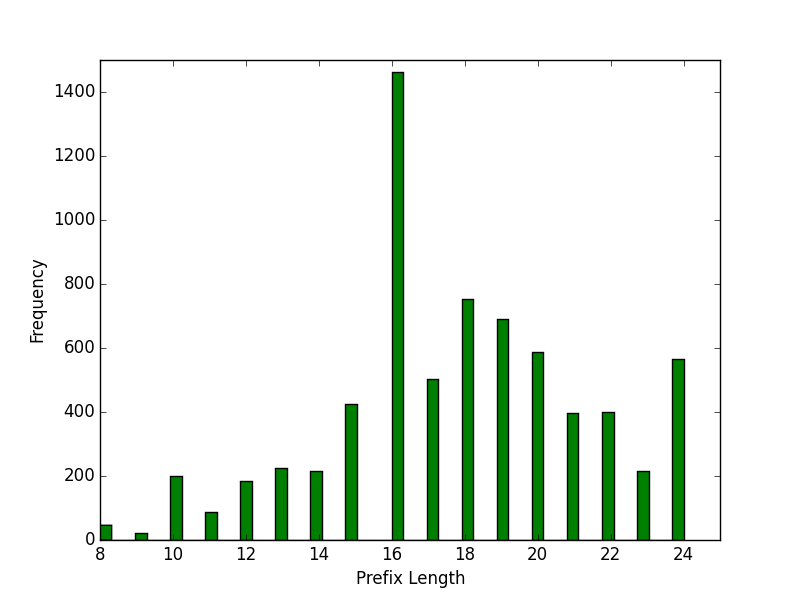
\includegraphics[width=80mm]{prefix_len_graph}
%\caption{Distribution of Tor bandwidth to Prefix Lengths \yixin{we need to fix this plot} \label{fig_prefixlen}}
%\end{figure}

Therefore, one way to defend against more-specific prefix hijack attacks is to move Tor guard relays into /24 prefixes. One concern that may arise is the extra burden which can be created on the routing table if announcing /24 prefixes for all Tor guard relays. We obtained a snapshot of the routing table from RouteViews ~\cite{routeviews}, and the Tor consensus data from January 2016. We found that there are 607,335 unique prefixes in the routing table, whereas there are only 1484 unique /24 prefixes covering all Tor guard relays (roughly 0.24\% of the routing table prefixes). Thus, the impact on the routing table size would be negligible. 

To make real world impact of this approach, we start a campaign in progress by contacting Tor relay operators, and suggesting that they move their Tor relays into /24 prefixes. We start with cooperating with an anonymous Tor relay operator, which contains a Tor relay under a /16 prefix. The approach they took was to announce an additional /24 prefix that covers the Tor relay, while still maintaining the original /16 announcement. This minimized the amount of work needed to move Tor relays into /24 prefixes. 

\subsection{Guard Relay Selection}
\label{subsec:relayselection}

Guard relays are at an important position in the Tor circuit, since they have direct connections with Tor clients. Section ~\ref{subsec:24prefix} discusses how to mitigate more-specific prefix hijack attacks; however, even if the guard relay belongs to a /24 prefix, it is still subject to an equally-specific prefix hijack attack. We have shown in Section \ref{hijack_interception_measurement} that high-bandwidth Tor relays could belong to ASes with low resilience to prefix hijack attacks, which put many Tor users at risk. Therefore, we propose a new guard relay selection algorithm that incorporates AS resilience in order to mitigate such active prefix hijacks on Tor.

%It has been shown that network-level adversaries can launch a more-specific BGP prefix attack to hijack the Tor traffic from the guard relay to the malicious AS \cite{sun2015raptor}. This can be potentially prevented by advertising /24 prefixes, as discussed in Section ~\ref{subsec:24prefix}. However, even if the guard relay belongs to a /24 prefix, it is still subject to an equally-specific prefix attack. Unlike more-specific attacks which spread through the whole internet, equally-specific attacks can only affect connections within a small range - i.e., ASes that have more preferred paths to the hijacking AS than the true origin AS. Thus, picking a Tor guard relay that has relatively high AS resiliency against such equally-specific attacks could protect Tor clients from being affected and deanonymized by network-level adversaries. Therefore, we propose a new guard relay selection algorithm that incorporates this aspect.

\subsubsection{Design Goals}
\begin{enumerate}
\item \emph{Mitigate prefix hijacks on Tor.} This is the main goal of the new guard relay selection algorithm. The algorithm computes the AS resilience against prefix hijacks of all Tor guard relays from the client source AS, and prefers the ones that have higher resilience, minimizing the likelihood that the client would be affected by a prefix hijack on its guard relay. 
\item \emph{Protect the anonymity of Tor clients.} In addition to lowering possibilities of being hijacked, the algorithm should also protect the anonymity of Tor users by balancing preferences among relays and providing rigorously assessed anonymity bounds. 
\item \emph{Performance and Load balancing.} The algorithm should incorporate relay bandwidth into the selection decision and avoid causing excessive traffic congestion on low bandwidth relays.
%\item \emph{Performance overhead.} The algorithm should have a reasonable performance overhead over the vanilla Tor algorithm when bootstrapping, and fast page load time. 
\end{enumerate}

\subsubsection{Mitigate Prefix Hijacks on Tor}

In Section \ref{hijack_methodology}, we measured AS resilience of each Tor-related AS based on the metrics proposed by~\cite{lad2007understanding}. The algorithm computes \emph{total} resilience of an AS by summing individual resiliencies from each source AS. \emph{However, the Tor client would only care about the individual resilience to a Tor-related AS from the source AS where the client is located}. Thus, instead of computing the total resilience, we use Algorithm ~\ref{algo:calcres} to calculate resilience $R(i)$ of each Tor-related AS $i$, from the client AS $t$. 

Tor relay selection is bandwidth-aware and prefers high bandwidth relays. The probability of each relay $i$ being chosen is based on its bandwidth $B(i)$. Thus, in order to still provide clients with the load balancing option of Tor bandwidths, we offer a tunable parameter $\alpha$ in the relay selection algorithm combining AS resiliency $R(i)$ and bandwidth $B(i)$. Each relay $i$ will be assigned a weight as following:
\begin{equation*}
W(i) = \alpha \times R(i) + (1 - \alpha) \times B(i)
\end{equation*}
Note that, when $\alpha$ is set to $0$, the relay selection becomes the same as bandwidth-only selection; while when $\alpha$ is set to $1$, the selection becomes resiliency-only selection. 

\subsubsection{Randomization is needed}
\label{relay_randomization}
If we simply select the set of guard relays based on the probability of $W(i)/\sum W(i)$, an adversary can potentially run a relay that has an AS-level path with high local preferences and/or short path length to the Tor client, such that it has high resilience from the client AS as the source. And it therefore obtains a high probability of being chosen. Furthermore, the Tor client might also be susceptible to fingerprinting attacks due to the differences in relay selection probabilities based on the AS-location of the client. An adversary that can observe the client for a long enough time may be able to infer the AS-location of the client based on its observed relay selection choices. Thus, we need to take into account these potential vulnerabilities and protect the anonymity of clients. Note that the weight of a Tor relay depends on two components: (1) the resilience of the AS in which the relay is located, and (2) the relay's bandwidth. The relay's bandwidth is not specific to client locations, and thus would not reveal any client identities; in addition, due to resource constraints, it is not trivial to run a relay with significantly higher bandwidth than all other relays to obtain high probability of being chosen. While on the contrary, AS resilience of relays \emph{is} client-specific, and requires much fewer resources to run a malicious relay with high AS resilience.

Instead of using resilience $R(i)$ for relay $i$ directly in the weight calculation, we first adjust it to $R(i)\prime$ by calculating the estimated inclusion probability of the relay in a random sampling of size $(g \cdot N)$ using the algorithm proposed by Tille ~\cite{tille1996elimination}. Note that $N$ corresponds to the total number of ASes containing Tor guard relays, and $g$ is a configurable parameter indicating the percentage of random sampling we want to perform. The steps are as following:
\begin{enumerate}
\item For each relay $i$, $R(i)\prime = \frac {k \cdot R(i)} {\sum R(i)}$ in which $k$ is initially equal to the sample size $(g \cdot N)$.
\item For each relay $i$, if $R(i)\prime > 1$, $R(i)\prime = 1$ and $k = k - 1$.
\item Repeat the above process until each $R(i)\prime$ is in $[0,1]$.
\item For each relay $i$, $R(i)\prime = \frac{R(i)\prime} {g \cdot N}$
\end{enumerate}

%performing a pseudorandom sampling without replacement using algorithm proposed by Tille (cite here). We compute the inclusion probability of each relay $i$ into a sample of size $(g \cdot total\_TorASes)$ given the fraction of its resilience $R(i)$ over total resiliences $\sum R(i)$, and then divide the inclusion probability by sample size $(g \cdot total\_TorASes)$ to get the probability of being chosen randomly within the sample. So the new resilience weight becomes:
%
%\begin{equation*}
%R(i) \prime = \frac {\pi(i | (g \cdot N))} {g \cdot N}
%\end{equation*}
%
%in which $\pi(i | m)$ represents inclusion probability of relay $i$ given sample size $m$, and $N$ is the total number of ASes that Tor relays reside in. $g$ is a configurable parameter indicating the percentage of random sampling we want to perform in the Tor-related AS set. 

Note that when $g$ is set to $0$, then no random sampling will be performed, while if $g$ is set to $1$, then all relays will have the same $R(i)\prime$ in their weights. 

%Instead of selecting relay directly based on its weight, we will first select a cluster of 
%\begin{equation*}
%m + \alpha \cdot g \cdot (N - m)
%\end{equation*}
%number of relays, in which $m$ is the minimum number of relays needed (i.e., 1 for single guard and 3 for multiple guards), $N$ is the total number of relays and $g$ is a configurable parameter indicating the maximum percentage of additional relays we want to pick into the cluster. Then, we will pick the guard relay(s) at random from the cluster. Note that when $g$ is set to $0$, then no additional randomization will be performed, while if $g$ is set to $1$, all guard relays will be picked randomly regardless of bandwidth or resiliency. We will evaluate how different values of $g$ may impact the security and anonymity.

\subsubsection{Implementation on Tor}
Mapping the IP addresses of the Tor client and Tor relays to their respective AS is necessary before we can compute AS resilience. In order to preserve the anonymity of the Tor client and not reveal its location to outside servers or anyone who can observe it's communications, the client will perform the IP to ASN mapping locally by utilizing the Maxmind ASN database ~\cite{maxmind}, which can be included in the Tor download package. Note that the vanilla Tor client uses the Maxmind GeoIP database for IP to Country mapping, which is already included in the Tor package as well. In addition, the client will use the AS topology database from CAIDA \cite{caida} for AS-level path inference in the resilience calculation. 

If the Tor client specifies in the torrc configuration file that the AS resilience-aware guard relay selection is preferred, and supplies an $\alpha$ value as the tunable parameter, the following procedure will be invoked:

\begin{enumerate}
\item If the Maxmind ASN file and AS topology file have not been downloaded, the Tor client will download the two files from Maxmind and CAIDA, respectively, and save them in the local data directory. 
\item The Tor client will perform IP to ASN mapping, and compute the AS resilience $R(i)$ of all candidate relays from the client AS as the source AS. 
\item The Tor client will perform random sampling on all ASes containing candidate relays and adjust the resilience value to $R(i)\prime$.
\item The Tor client will compute a weight for each candidate relay using formula $W(i) = \alpha \times R(i) \prime + (1 - \alpha) \times B(i)$. 
%\item The Tor client will select a cluster of $m + \alpha \cdot g \cdot (N - m)$ relays based on their weights, and then randomly select the guard relay(s) from the cluster. 
\item The Tor client will proceed with the path selection. The remaining part of the circuit construction process stays the same as it is in Tor. 
\end{enumerate}

\subsection{Security and Anonymity Evaluation}
We evaluate the security and anonymity of the Tor guard relay selection algorithm from three perspectives: (1) reduction in probability of a Tor client being affected by a hijack attack on the Tor guard relay, (2) balancing preferences in relay selection to avoid favoring certain relays significantly more than the others, (3) vulnerability to client fingerprinting attacks, and (4) rigorously assessed anonymity bound for a given Tor client. 

\subsubsection{Probability of a Tor client being affected by a hijack attack on Tor guard relay}
\label{attack_probability}
This is the main goal of the new relay selection algorithm. Let $P_{pick}(i)$ denotes the probability that a Tor client will choose relay $i$ using our algorithm, and $P_{deceived}(i)$ denotes the probability that a Tor client will be deceived if relay $i$ is being hijacked. $P_{deceived}(i)$ can be calculated using similar method in Section ~\ref{hijack_interception_measurement}, the details of which will be addressed in the Appendix. The overall probability of a Tor client being affected by a hijack attack on guard relay can then be expressed as:
\begin{equation*}
\sum_{i \in \{all guard relays\}} P_{pick}(i) * P_{deceived}(i)
\end{equation*}

We first evaluate the probability without random sampling for five values of $\alpha=\{0, 0.25, 0.5, 0.75, 1\}$ with $1000$ randomly selected ASes as the source AS and Tor consensus data from January 2016. Figure ~\ref{fig_attack} shows the result. Table ~\ref{tbl_attack_reduction} shows the average percentage of reduction in the probability of being affected by a hijack attack compared to $\alpha=0$. We can see that $\alpha=1$ has the lowest probability of being affected by an attack, with an average of 31\% reduction. 

\begin{figure}[ht!]
\centering
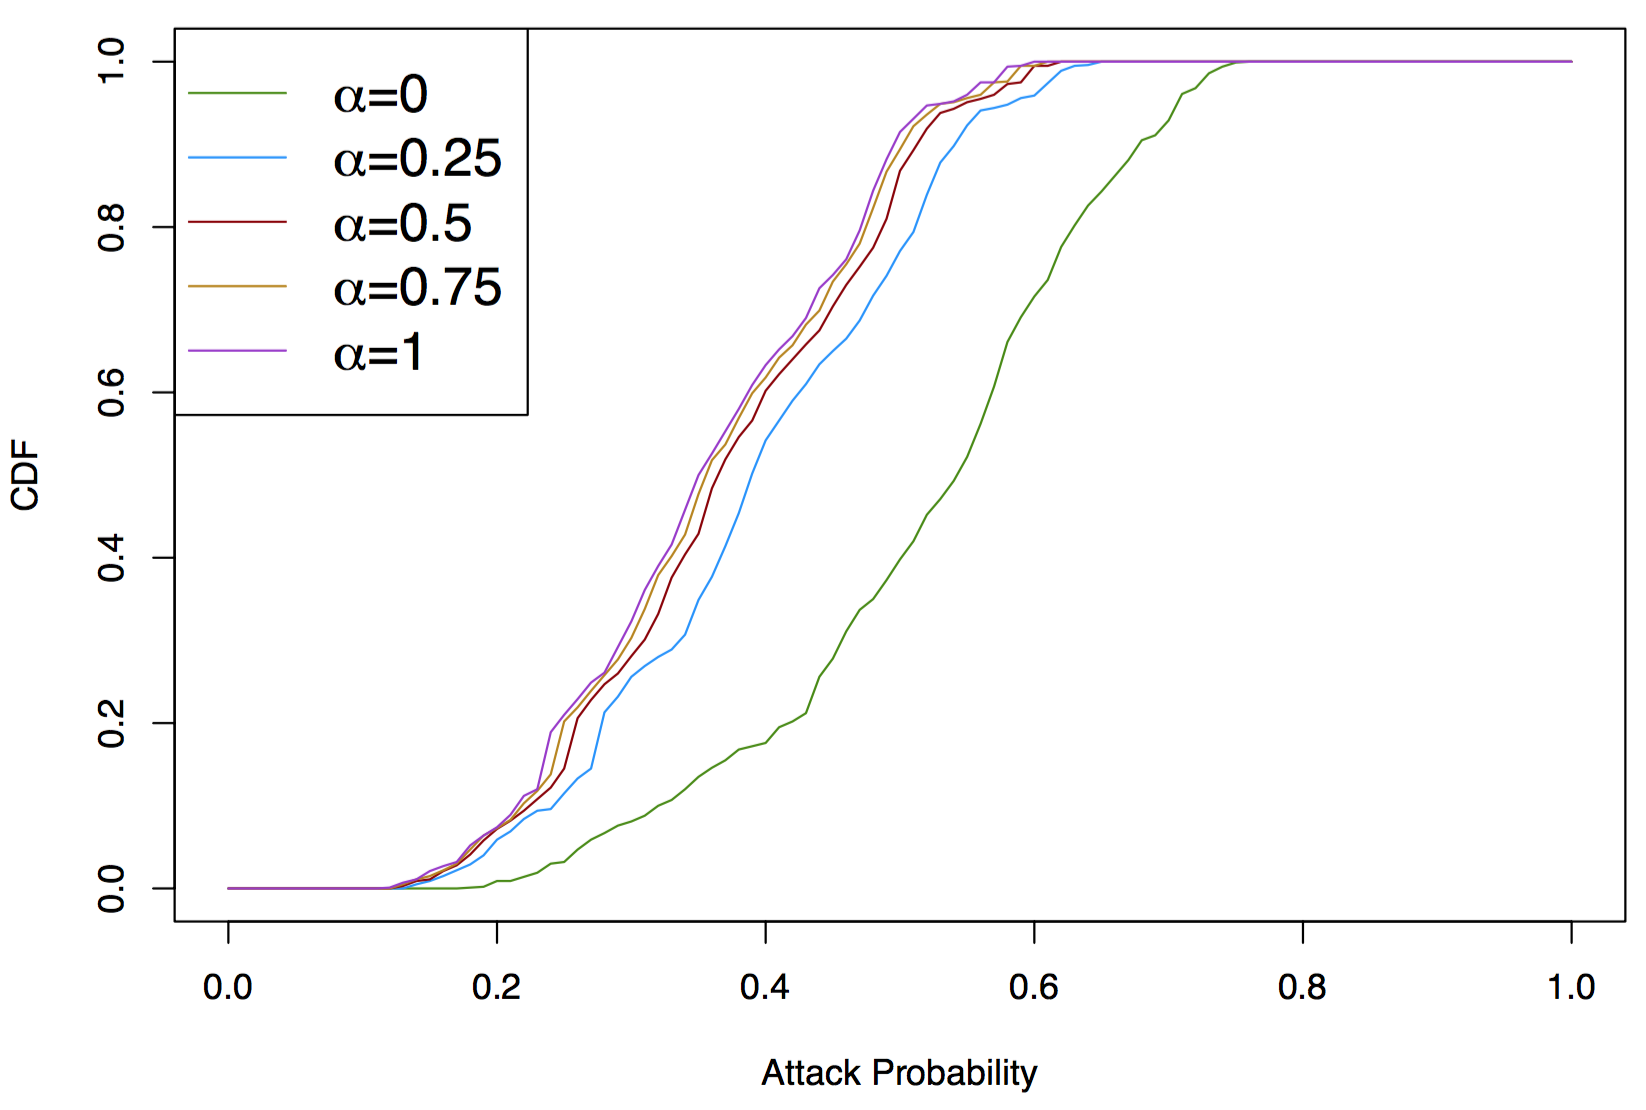
\includegraphics[width=80mm]{figure/attack}
\caption{Attack Probability with different $\alpha$ values \label{fig_attack}}
\end{figure}

%in probability for the $1000$ client ASes compared to $\alpha=0$. When $\alpha=0.25$, the probability increases a bit, with an average of 24\% reduction compared to $\alpha=0$. While $\alpha=\{0.5,0.75\}$ has similar probability to $\alpha=1$, with average of 28\% and 30\% reduction in probability, respectively. 

We then evaluate it with random sampling of $g=10\%$. Figure ~\ref{fig_attack_random} shows the comparison of $\alpha=\{0.25, 0.5\}$ with and without random sampling. Table ~\ref{tbl_attack_reduction} shows the average percentage of reduction in attack probability with $g=10\%$ random sampling. We can see that there is only a very slight decrease in the reduction percentage with the random sampling. 

\begin{figure}[ht!]
\centering
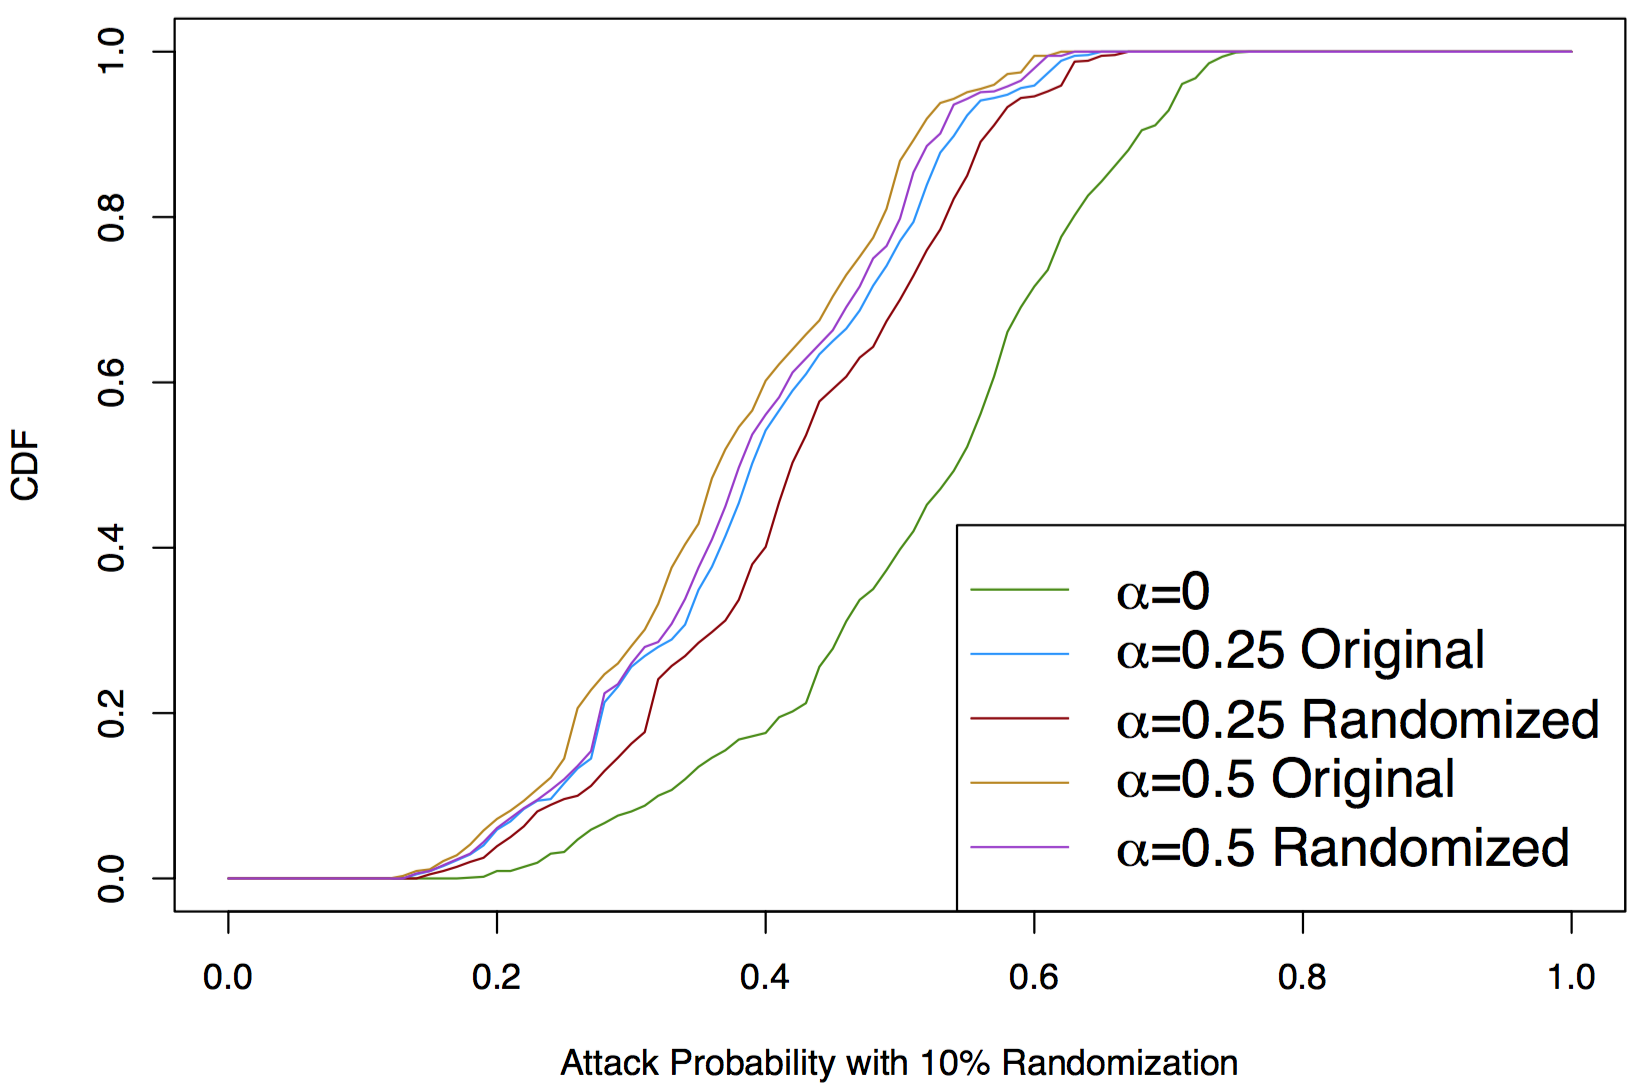
\includegraphics[width=80mm]{figure/attack_randomize}
\caption{Attack Probability with $g=10\%$ sampling \label{fig_attack_random}}
\end{figure}

\begin{table}[ht!]
\begin{center}
 \begin{tabular}{ p{5mm} | p{2.5cm} | p{2.5cm}}
    \hline
    $\alpha$ & Without Random Sampling & With  $g=10\%$ sampling\\ \hline
    0.25 & 24\% & 19\% \\
    0.5 & 28\% & 25\% \\
    0.75 & 30\% & 29\% \\
    1 & 31\% & 31\% \\
    \hline
  \end{tabular}
\end{center}
\caption{Percentage of reduction in attack probability compared to $\alpha=0$ \label{tbl_attack_reduction}}
\end{table}

\subsubsection{Balancing Relay Selection Preferences} 
We want to main good balance among the weights/preferences for each candidate relay to avoid strongly favoring certain relays over the others. For instance, for a given Tor client, if relay $i$ has 90\% probability of being chosen while all other relays totals up to 10\% probability, then this can create potential security vulnerabilities, let alone performance issues. An adversary may easily target relay $i$ to launch an attack, or even manipulate the selection algorithm to strongly favor a relay run by the adversary. Thus, we want to evaluate the variance in probabilities of a given Tor client picking any particular relay and show that it's well-balanced. 

We used Gini coefficient as the variance evaluation metric, as it has been used in previous work ~\cite{akhoondi2012lastor}. We first evaluate without random sampling, for five values of $\alpha: \{0, 0.25, 0.5, 0.75, 1\}$ with $1000$ randomly selected ASes as source AS and Tor consensus data from January 2016. Figure ~\ref{fig_gini} shows the result. The green line to the right is when $\alpha = 0$, which is solely based on bandwidth, resulting in a Gini coefficient of $0.51$ for all source ASes. The Gini coefficients for the other four $\alpha$ values which involve resilience-based selection are much lower than bandwidth-only selection, meaning that there is lower skew in probability of selecting any particular relay and thus is more well-balanced. 

\begin{figure}[ht!]
\centering
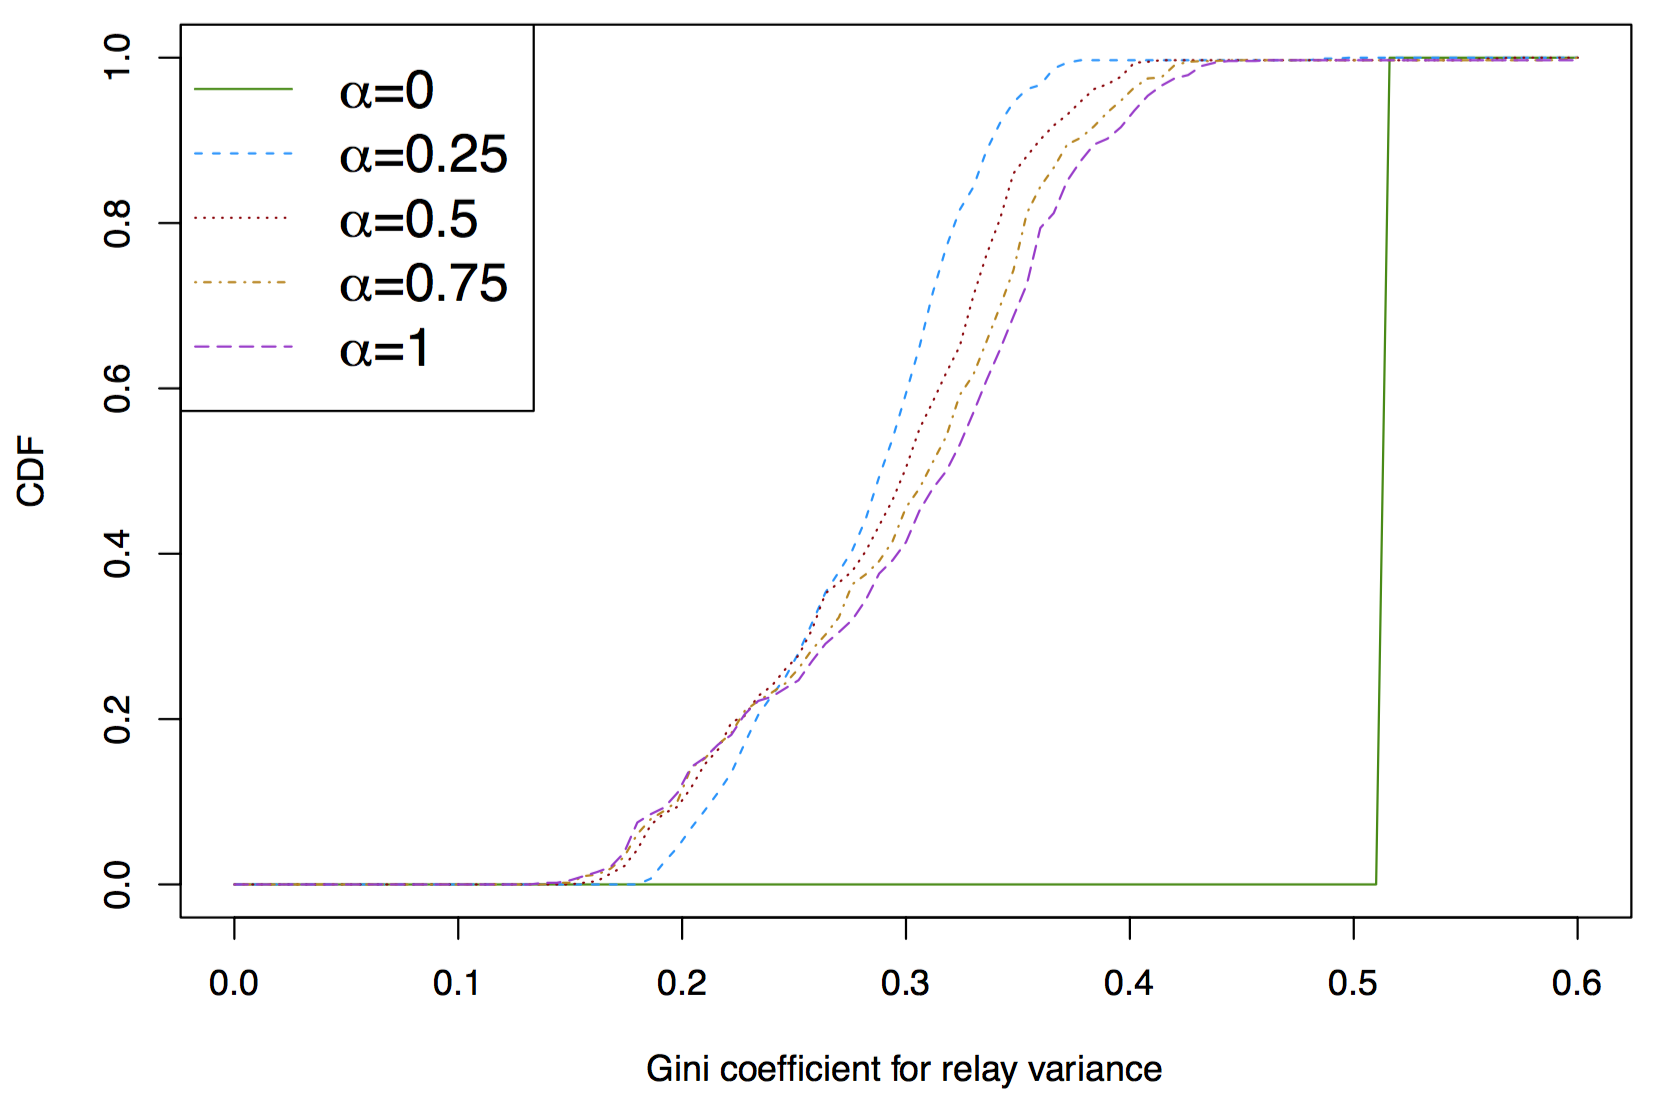
\includegraphics[width=80mm]{figure/gini_relay_variance}
\caption{Gini coefficients for variance in relay selection preferences given a Tor client. Lower Gini coefficient value indicates higher variance and less skew. \label{fig_gini}}
\end{figure}

\subsubsection{Vulnerability to client fingerprinting attacks}
This is a potential security tradeoff of the relay selection algorithm. We briefly discussed in Section ~\ref{relay_randomization} about fingerprinting a client location based on its preferences of relays in the long term. For instance, for a given relay, if client $a$ has 70\% probability of choosing the relay while client $b$ only has 30\% probability, then an adversary can observe the client's choice of relays overtime to infer client information. The resilience component of our relay selection algorithm may be subjective to such fingerprinting attacks, which we will evaluate here. 

We used Gini coefficient again as the variance evaluation metric, but evaluating \emph{the variance in the probability of each client choosing a given relay} instead. Figure ~\ref{fig_gini_client} shows the result for $1000$ randomly selected ASes as client AS. 

We can see that the bandwidth-only selection in Vanilla Tor ($\alpha = 0$) has perfect Gini coefficient value of 0 for all relays, since given a relay, the probability of it being chosen is the same across all clients. With resilience-based selection, the skews in probabilities are higher. When $\alpha = 1$ (resilience-only), $80\%$ of the relays have coefficients $> 0.4$. This skew in probability might be exploited by adversaries who can observe the client over a period of time to infer client locations given the differences in relay selection.

We then evaluate it again with $g=10\%$ random sampling. Note that since $\alpha=\{0.75,1\}$ does not have a significant advantage in attack resilience over $\alpha=\{0.25,0.5\}$ in Section ~\ref{attack_probability}, while resulting in higher skew in probabilities, so we focus on evaluating the later here. Figure ~\ref{fig_gini_client_random} shows that by performing $10\%$ random sampling, when $\alpha=0.25$, $80\%$ of the relays have coefficients reduced to $< 0.28$. Although this may still pose some vulnerability to client fingerprinting, we argue that since Tor clients only select guard relays at bootstrapping time, and would then use the same guard relays over several months or until the relays become unavailable, so fingerprinting the client could not be done in a reasonably short time, especially given the low variance of probabilities (although not perfect) as shown.


\begin{figure}[ht!]
\centering
\begin{subfigure}{.25\textwidth}
\centering
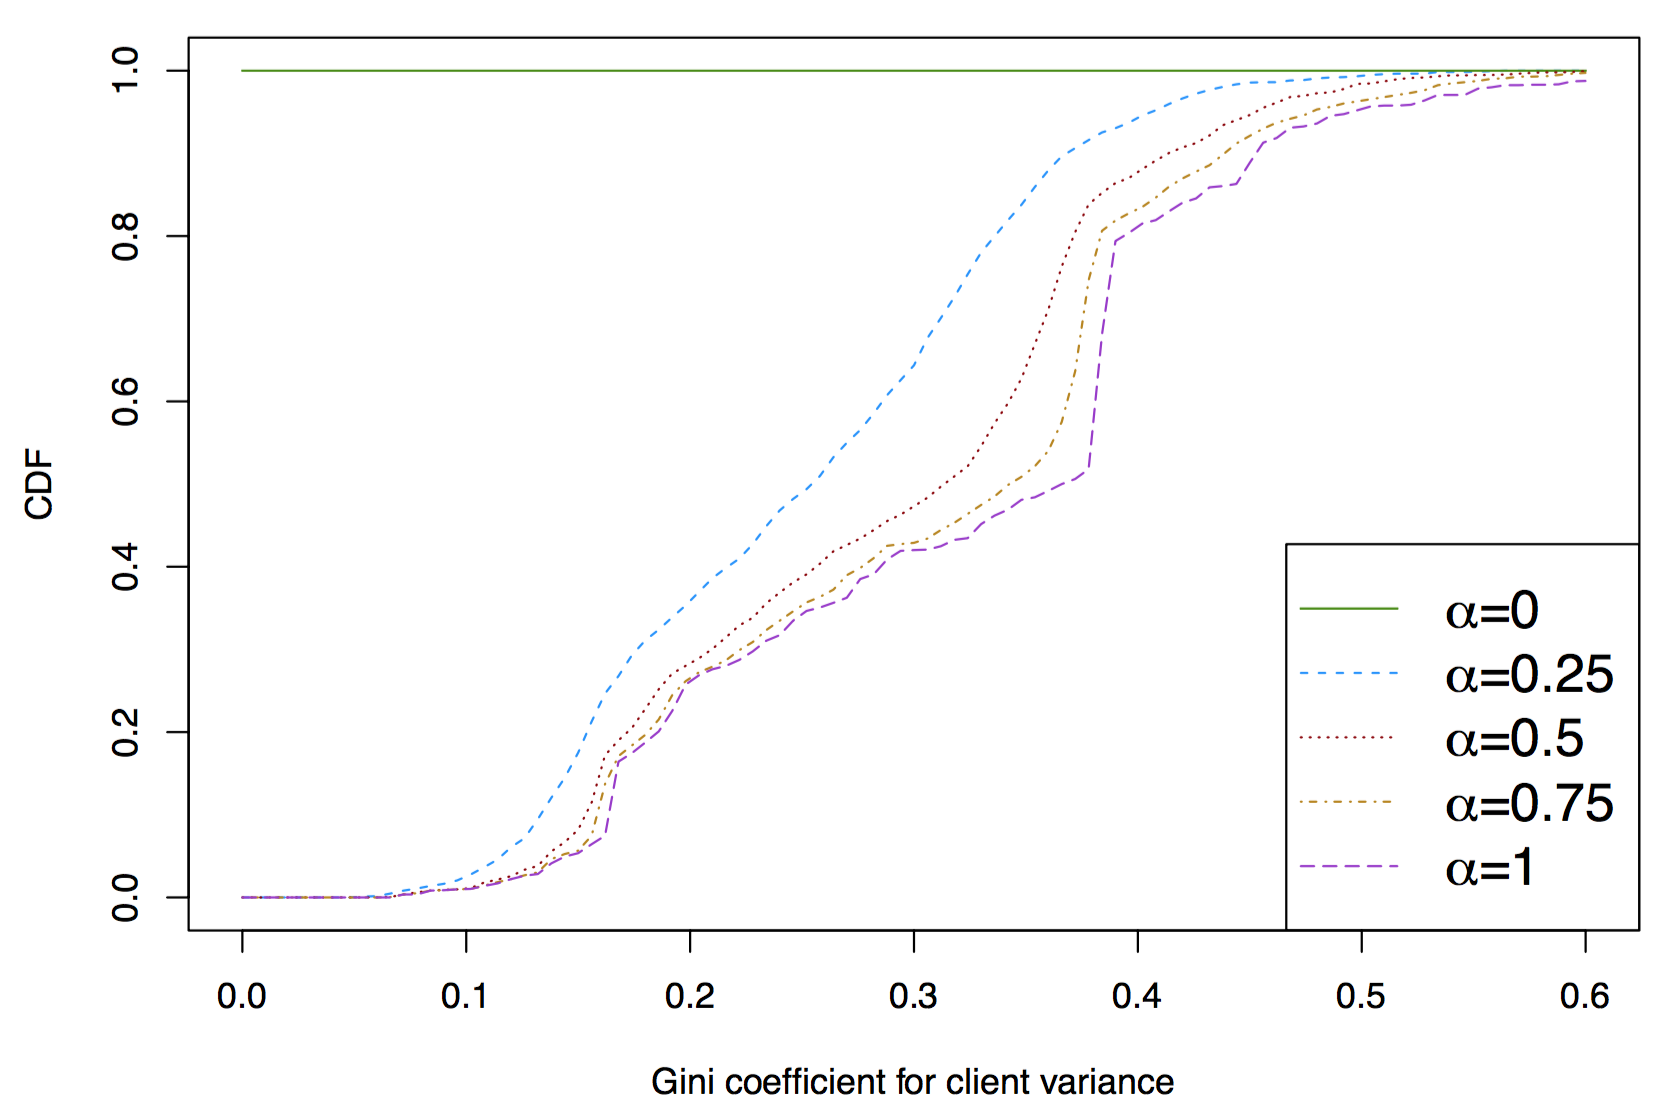
\includegraphics[width=.9\linewidth]{figure/gini_client_variance}
\caption{Without random sampling \label{fig_gini_client}}
\end{subfigure}%
\begin{subfigure}{.25\textwidth}
\centering
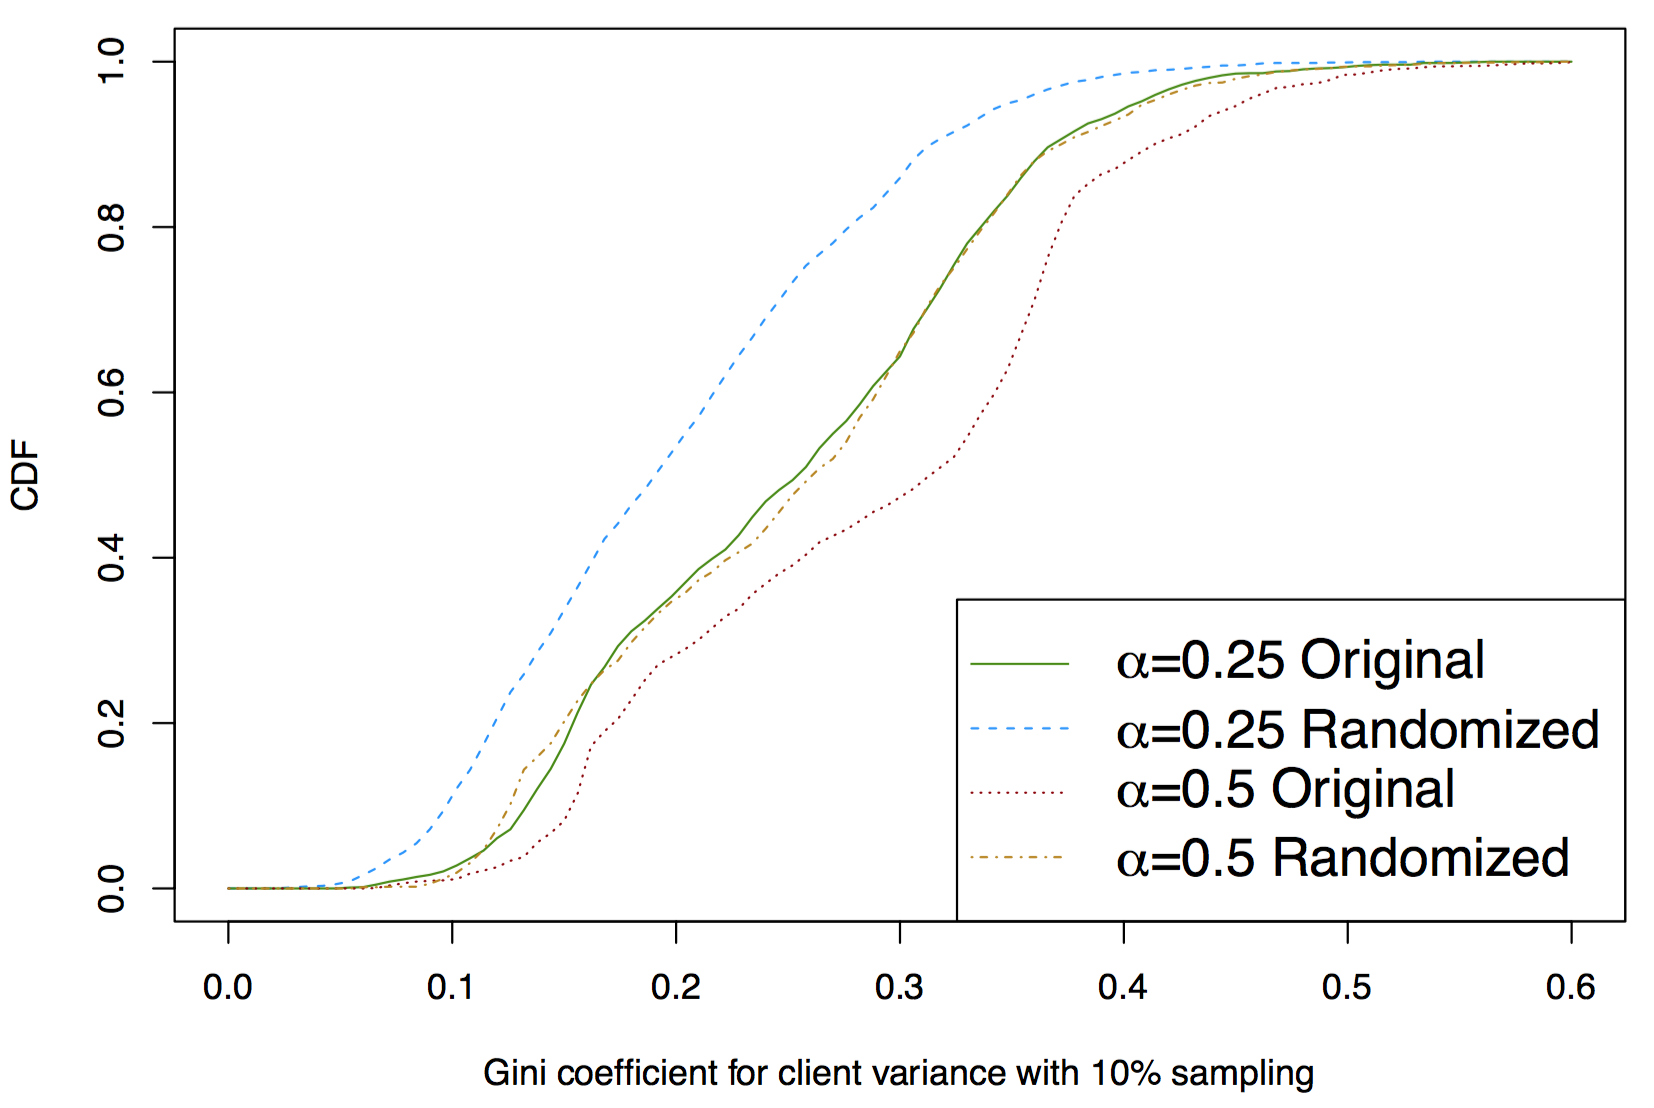
\includegraphics[width=.9\linewidth]{figure/randomize_client_gini}
\caption{With $g=10\%$ sampling \label{fig_gini_client_random}}
\end{subfigure}
\caption{Gini coefficients for variance in client's probability of choosing a given relay.}
\label{fig:gini_client}
\end{figure}

\subsubsection{Formal anonymity assessment}
Finally, we evaluate the anonymity of a given Tor client using MATor, a framework for assessing the degree of anonymity in Tor with rigorously proved anonymity bounds ~\cite{backes2014nothing}. We implemented our new relay selection algorithm into MATor source code, and evaluated it in comparison with vanilla Tor. Note that we picked the top Tor client location AS6128 ~\cite{juen2012protecting} to evaluate here. We used default configuration of multiplicative factor $\epsilon=1.3$, ports setting of HTTPS+IRC vs. HTTPS, and $0.5\%$ of total nodes as compromised nodes. We evaluated using Tor consensus files from 2/1/2016 - 2/9/2016 and server descriptor from February 2016. Figure ~\ref{fig_mator} shows the result. 

\begin{figure}[ht!]
\centering
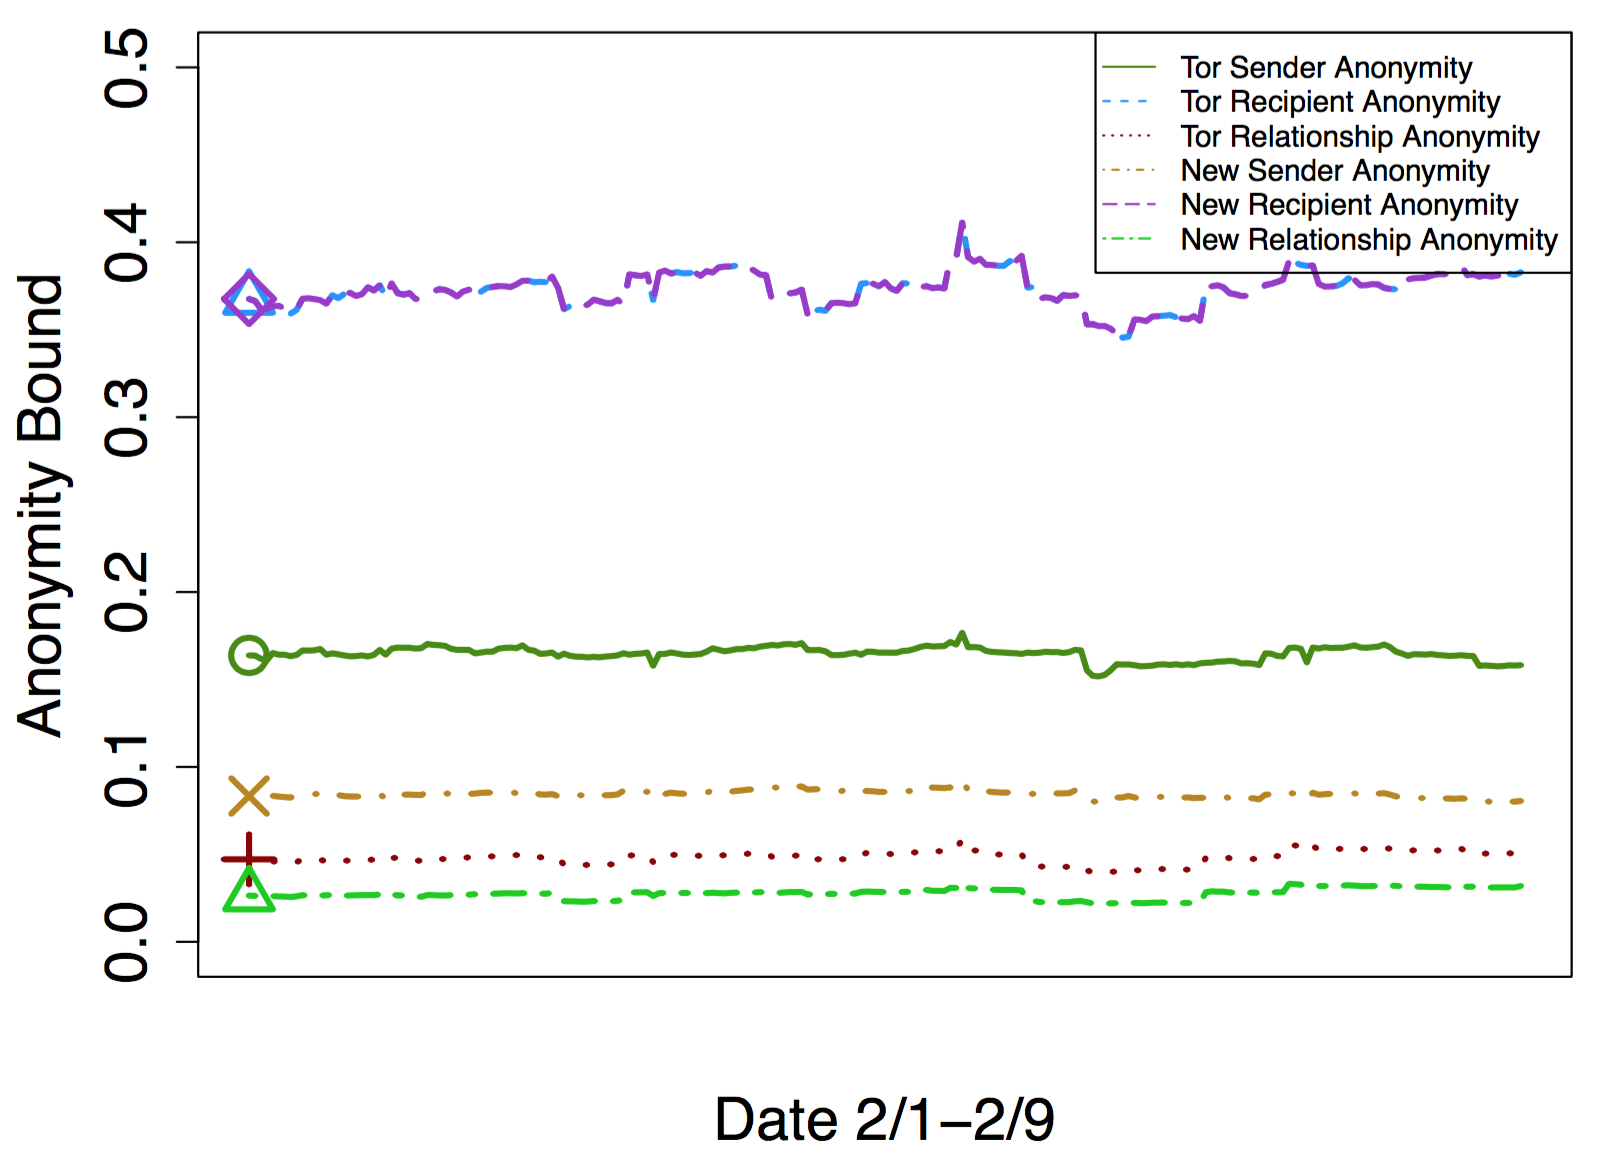
\includegraphics[width=80mm]{figure/mator}
\caption{MATor Anonymity Bound 2/1/2016 - 2/9/2016\label{fig_mator}}
\end{figure}

MATor evaluates three anonymity notions (sender, recipient, and relationship anonymity). The full details of the anonymity definitions are described in ~\cite{backes2014nothing}. The result shows that our new guard relay selection has tighter anonymity bounds on sender and relationship anonymities compared to current Tor path selection, indicating better anonymity guarantees. The recipient anonymity remains the same as vanilla Tor, which is expected since we do not alter selection algorithm for exit relays. 


%However, the variance in relay selection probability \emph{across} different source ASes is bigger than bandwidth-only: when $\alpha = 0$, all sources ASes have the same gini coefficient of $0.607$, while for other $\alpha$ values, the gini coefficient could vary from approximately $0.2$ to $0.4$, depending on the source AS. 


\subsection{Performance Evaluation}

We first evaluate the runtime of the AS resilience calculation given a source AS. We pick $1000$ ASes randomly as the source AS, and record how much time it takes each of them to complete the calculation. Most of the source ASes finish within $0.6$ second. \\

%\begin{figure}[ht!]
%\centering
%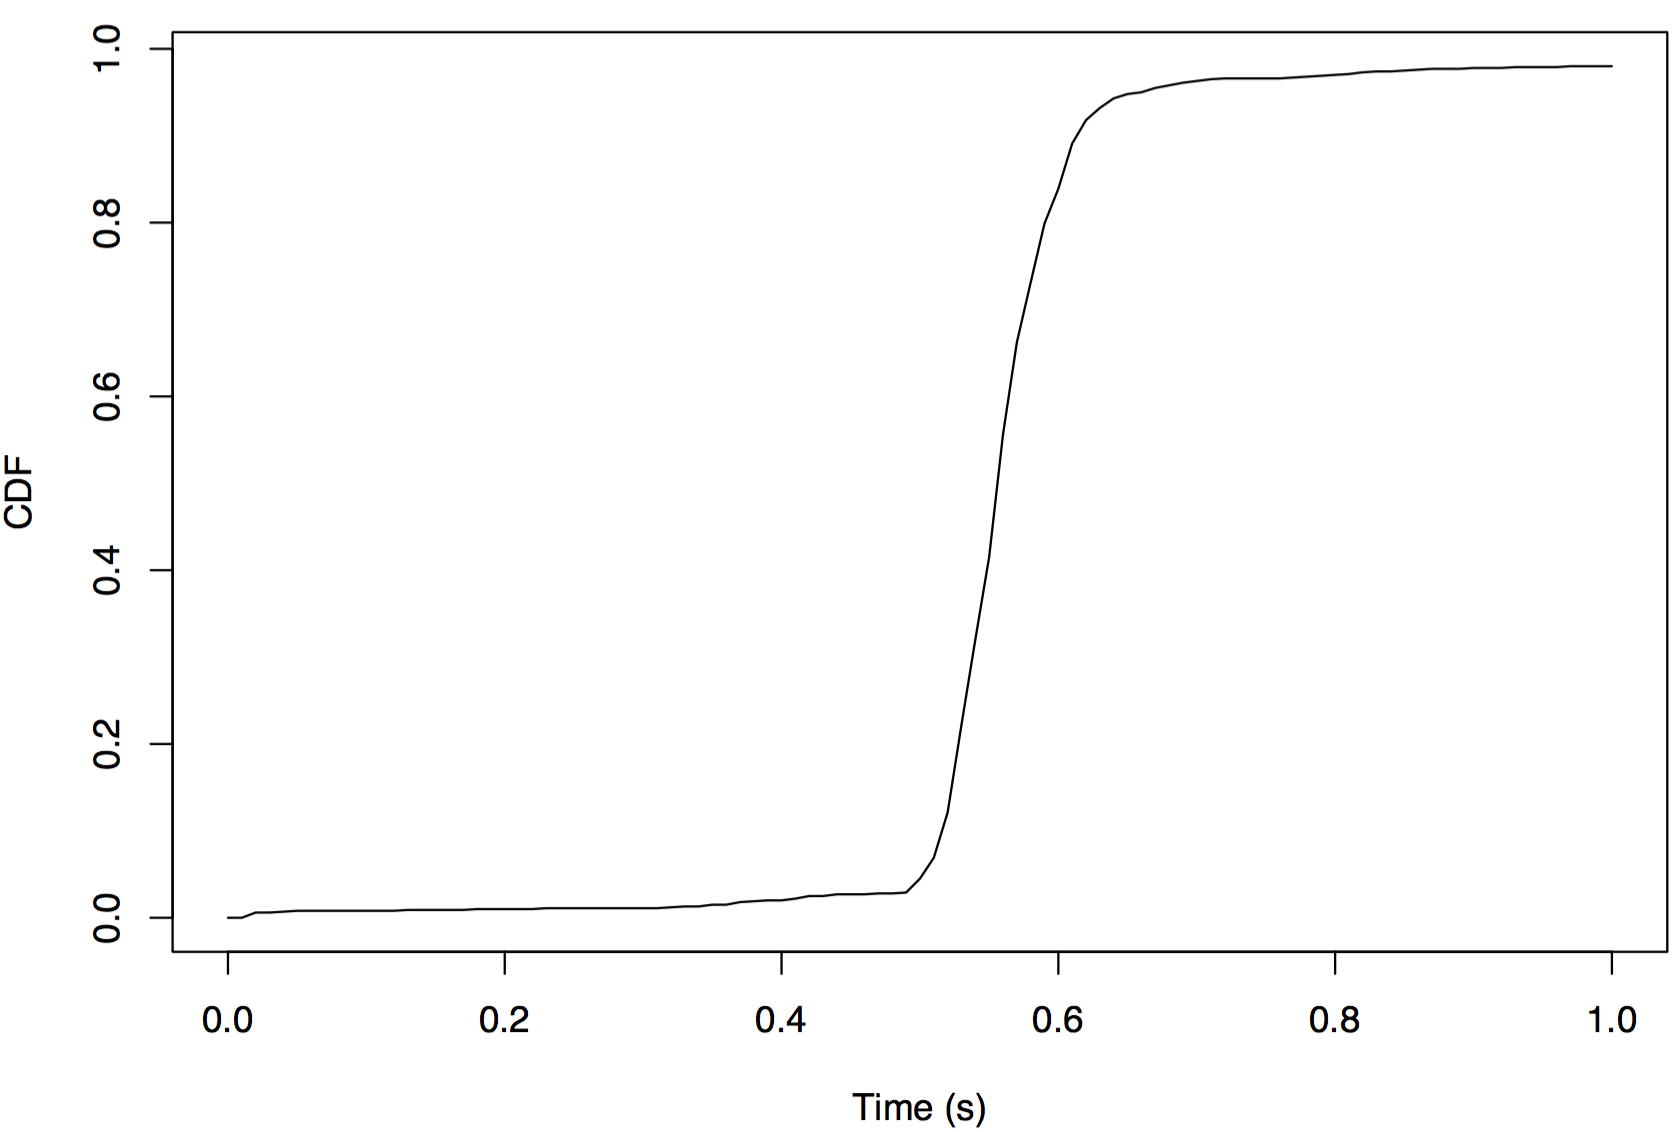
\includegraphics[width=80mm]{figure/runtime}
%\caption{Runtime of AS resilience calculation from a given source AS \label{fig_ascal}}
%\end{figure}

Next, we installed our new Tor client on $26$ Planetlab nodes located in different ASes, and performed page loads of Alexa top 100 websites. We compared the performance of $\alpha=\{0.25,0.5\}$ with $g=10\%$ random sampling against vanilla Tor. Figure ~\ref{fig_pageload} shows the page load time. We can see that all three have very similar performance. This can be explained in the following ways. First, we do not restrict the relay selection to a smaller set of relays, but rather \emph{preferring} certain relays over the others; second, the $\alpha$ value was tuned to be $\{0.25,0.5\}$, which gives sufficient weight to the bandwidth in relay selection; thirdly, the relay selected has a relatively short AS path (and is likely geographically closer);finally, the algorithm is only for guard relay selection, whereas exit relay selection remains the same as purely bandwidth-weighted selection. These are some reasons why the new guard relay selection algorithm does not suffer any performance loss in page load time. 

\begin{figure}[ht!]
\centering
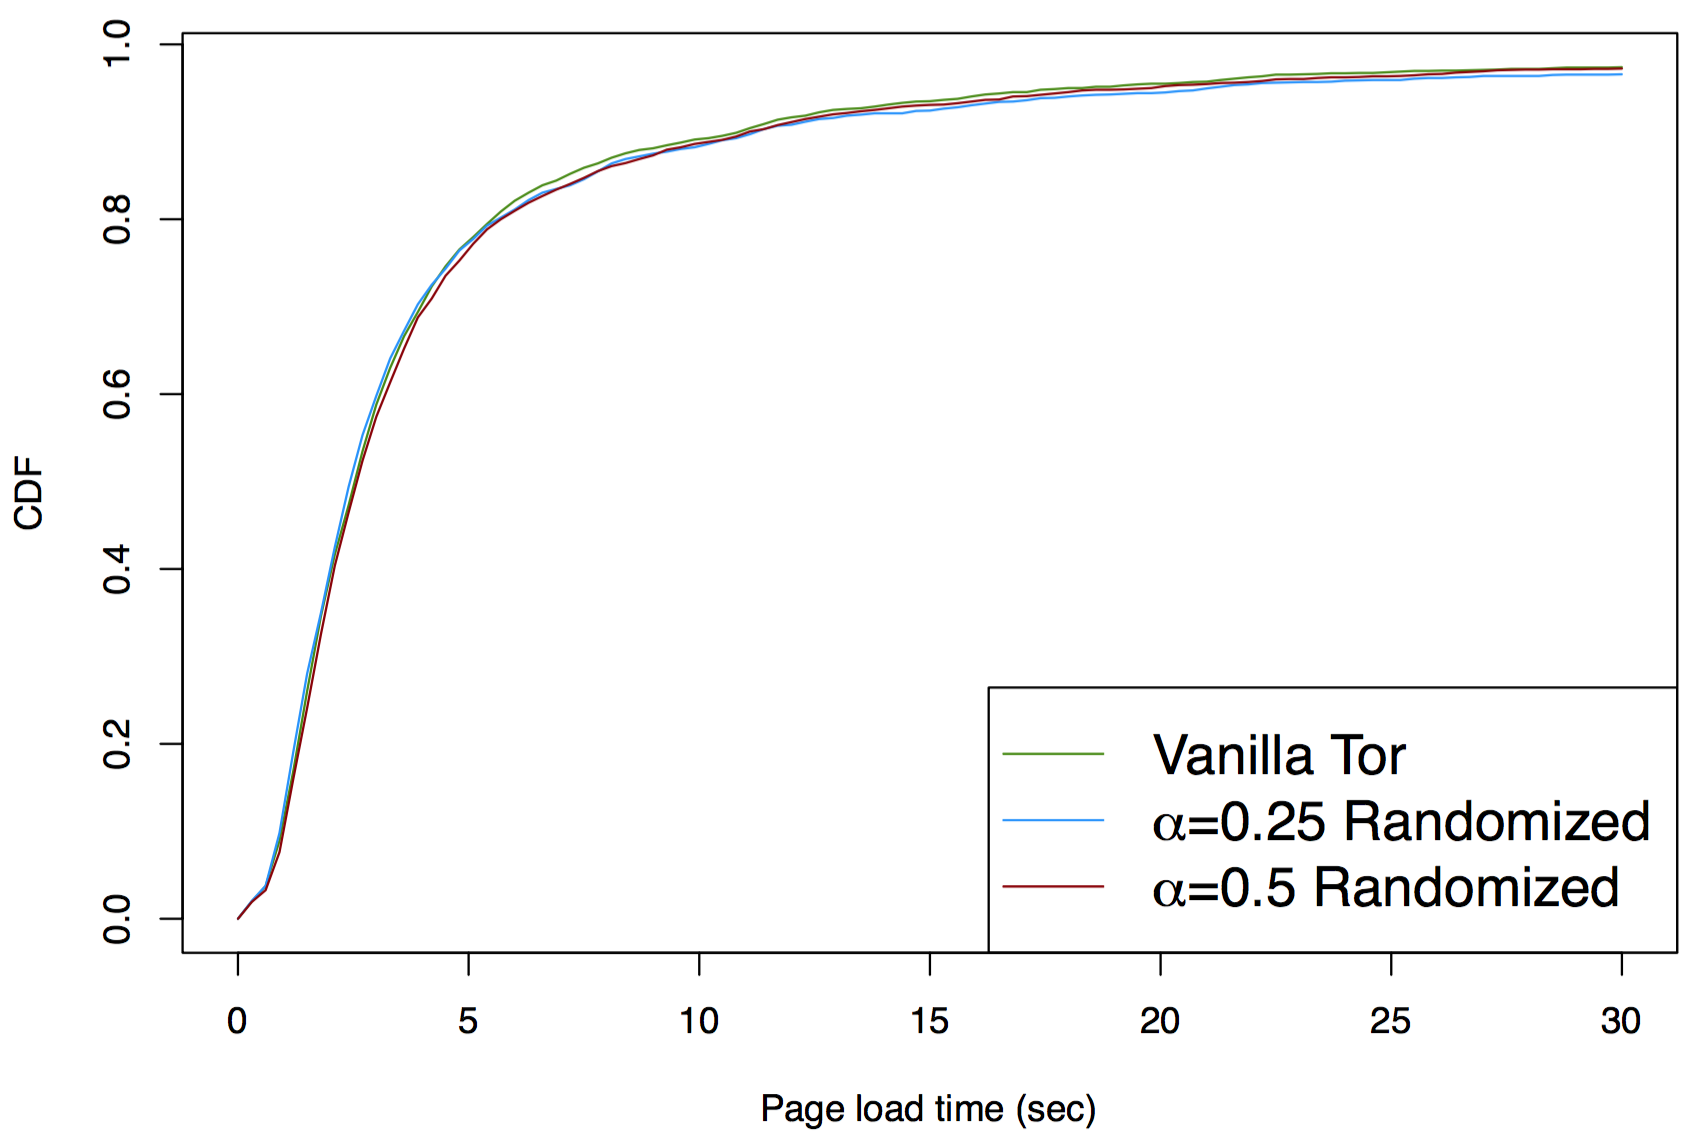
\includegraphics[width=80mm]{figure/pageloadtime}
\caption{Page load time of Alexa top 100 sites \label{fig_pageload}}
\end{figure}




\section{Reactive Approaches}
In addition to proactive approaches to helping prevent active BGP routing attacks, we have also taken a reactive approach.  In the case that an attack is happening, we can detect it using a live monitoring framework.

\subsection{A Live Monitoring Framework for Tor}
A possible countermeasure against routing attacks on the Tor network is attack 
detection and user notification.  Routing authorities then know which relays are 
being hijacked and/or intercepted, and can make routing decisions accordingly.  
We observed that routing attacks are almost always short-lived (CITATION HERE), which allows 
routing authorities to suspend use of hijacked/intercepted relays until enough 
time has passed to use them again.

The live monitoring framework aims at detecting suspicious routing attacks that affect Tor relays, and reacts correspondingly to alert Tor clients of the scenario. The monitoring framework consists of two parts: BGP monitoring and Traceroute monitoring.\\

{\bf Relay Info from Tor Consensus.} Tor consensus releases up-to-date information for current running relays every hour. Our system automatically fetches this consensus data once it's updated. We focus on guard relays and exit relays, which reside at the two ends of the communication path and can easily be the target of an adversary. Further more, since we focus on AS-level adversaries, it is unnecessary to monitor each individual relay by its IP address. Instead, we monitor the /24 prefixes which contain Tor guard and exit relays. Note that, there is no need to monitor a more specific prefix than /24, since generally /24 is the longest prefix accepted in BGP announcement. \\

%Thus, we construct a live monitoring database which is being updated every hour with latest Tor relay data. The table contains the following fields:
%\begin{center}
%\begin{tabular}{ p{8mm} | p{1.4cm} | p{1.3cm} | p{1.3cm} | p{1.3cm}}
 % \hline			
  %$/24$ Prefix & Total Bandwidth & Number of Guards & Number of Exits & Timestamp \\
  %\hline  
%\end{tabular}
%\label{tab:relayinfo}
%\end{center}
%Each /24 prefix that contains any guard/exit relays will have one entry in the table, and the list of /24 prefixes will be used for our BGP and Traceroute monitoring frameworks, which we describe in the following. 

{\bf BGP Monitoring Framework} monitors the control plane of internet routing. We collect live BGP announcements data from BGP Stream ~\cite{bgpstream}, in combination with the latest Tor relay data. We monitor all the Tor-related /24 prefixes we obtain, as described in the table above. We check if any activity related with the prefixes exhibit any anomaly. These anomalies can be detected by developing certain heuristics, such as the amount of time that a BGP path is used or the frequency that a path is announced; if certain anomalies fall under a threshold for a given heuristic, they should be flagged as potential attacks. This analysis will require saving inactive relay BGP info for some period of time.  This framework helps:

\begin{itemize}
\item Identify suspicious prefix announcements.
\item Differentiate between potential attacks and ``normal'' behavior, such as multiple origin AS conflicts, backup paths, etc~\cite{zhao2001analysis}.
\end{itemize}

We use Team Cymru ~\cite{teamcymru} to obtain AS ownership of prefixes. Some prefixes are owned by an organization with multiple AS numbers, so we take this aspect into consideration and store the AS origins of these prefixes. If we observe any change in AS paths, we will first check if the prefix has multiple AS origins, and if so, as long as the new on-path AS also owns the prefix, then it would not be seen as an attack. 

The implementation of the BGP Monitoring framework is based on BGP Stream~\cite{bgpstream}.  We analyze the live stream of BGP updates and withdrawals, focusing just on the prefixes that contain a Tor relay.  We monitor the prefixes that are reported through Team Cymru, as well as the /24 that contains each relay; we do this because we would like to be able to detect sub-prefix hijack attacks, so we must monitor longer prefixes in addition to the reported prefix.  

In addition to comparing the AS that owns a prefix (according to Team Cymru) with the AS that announces the prefix, our analysis involves three different detection techniques:

\begin{enumerate}
\item Origin AS check.  We collect the origin AS in the live BGP update and compare it to the owner AS reported by Team Cymru.  If these don't match up, then we flag the update (and prefix) as a potential hijack, otherwise we ignore it. 
\item Frequency heuristic.  Routing attacks can be 
characterized by an AS announcing a path once (or extremely rarely) to a prefix 
that it does not own.  The frequency heuristic detects attacks that exhibit this behavior. 
It measures the frequency of each AS that originates a given prefix; if the frequency is 
lower than a specified threshold, then it could be a potential hijack attack.
\item Time heuristic.  Most known attacks 
last a relatively short amount of time. The time heuristic measures the amount of time each 
path to a prefix is announced for; if the amount of time is extremely small (below a specified threshold), 
then there is the possibility of it being a routing attack. 
\end{enumerate}  

{\bf Traceroute Monitoring Framework} monitors the data plane of Internet routing, i.e., how packets travel through the Internet in reality. The traceroute monitoring framework is used as a verification mechanism if the BGP monitoring framework flags certain behavior. There may be many false positives in detecting hijack/interception attacks due to the nature of BGP.  With many false positives, the traceroute monitoring framework will be used often for verification - this raises a question of optimization, which we will also address.

Our Traceroute monitoring framework retrieves updated Tor relay data hourly from the Tor consensus as described above. Since running large number of continuous traceroutes to relay IP addresses may create unnecessary extra traffic to the Tor network, we selectively monitor a subset of prefixes when there is no anomaly from BGP monitoring data, and when there is suspicious activity report by BGP monitoring, the traceroute monitoring can be "triggered" to target the suspicious prefix announcement to verify the anomaly. 
\begin{itemize}
\item Selectively monitor relays of interest.\\
%A /24 prefix can be evaluated based on several factors: (1) total combined bandwidth of Tor relays it covers, denoted as $b_i$ for prefix $i$; (2) total number of guard relays it covers, denoted as $g_i$; (3) total number of exit relays it covers, denoted as $e_i$; and (4) resilience of the prefix to BGP hijack/interception attacks, denoted as $r_i$. These factors can make the prefix an attractive target to adversaries. Using these factors, we want to formulate the overall security of the system as following, and the goal is to find the monitoring frequency $f_i$ for each relay $i$ that maximizes the overall security of the network. \\
%\begin{align}
%\max \sum_{i=1}^N & \frac {\log {(f_i + 1)}} {b_i + g_i + e_i + r_i}\\
%\text{s.t. } &\sum_{i=1}^N f_i \leq F\\
%&0 < f_i \leq M, \forall i
%\end{align}
%$N$ is the total number of prefixes we want to monitor, $F$ is the constraint on total number of traceroutes we can send from each Planetlab node per day, and $M$ is the constraint on total number of traceroutes needed for each prefix. Given the solution, we use a collection of Planetlab nodes located in different ASes to send traceroutes to the prefix at its frequency rate. 
A /24 prefix can be evaluated based on (1) total combined bandwidth of Tor guard/exit relays it covers, and (2) total number of guard/exit relays it covers. These two factors can make the prefix an attractive target to adversaries due to the high amount of traffic it could be handling. Thus, we rank all the /24 prefixes by combining its cumulative bandwidth and number of relays, and selectively monitor the top 50 prefixes when there is no anomaly triggered by BGP monitoring framework. 
We use PlanetLab nodes that are located in different ASes (updated daily to get the latest list of PlanetLab nodes) to send traceroute requests to the prefixes hourly. We compare the current traceroute paths to previously recorded traceroute paths to detect any anomaly, which will be described in more details in the following. 

\item Monitoring target prefixes triggered by BGP.\\
If we detect any anomaly from the BGP monitoring framework, we will immediately send traceroutes to the suspicious prefixes to verify whether there is truly a path change happening on the data plane to the Tor relays. 

\item Detecting anomaly from Traceroutes\\
%Even when there is no suspicious activity reported by BGP monitoring, it is also possible we detect anomaly from our selective traceroute monitoring. 
We keep track of the past traceroute monitoring paths in a database table, as following:
\begin{center}
\begin{tabular}{ p{9mm} | p{9mm} | p{6mm} | p{1.2cm} | p{1.2cm}} %| p{8mm}}
  \hline			
  Source Prefix & Dest Prefix & AS Path & Time Created & Time Last Updated \\ %& Current \\
  \hline  
\end{tabular}
\label{tab:pathinfo}
\end{center}
Note that, instead of recording every hop in the traceroute path, we first convert the IP to ASN using Team Cymru whois server (citation here), and eliminate any duplicated intra-AS hops to obtain the final AS-level paths. With this table, we will be able to compare the current AS path with \emph{any} previously seen AS paths to detect any path changes. If there is any anomaly detected, we will log a warning and make it public. 

\end{itemize}

\subsection{Framework Evaluation}
The live monitoring framework will be evaluated on a number of characteristics, including false positive rate, false negative rate, as well as performance and overhead. \annie{We will add more evaluation here.}

\subsection{Deployment Experience}
The BGP monitoring framework has been running for a week.  It has recorded over 3 million announcements (not specific to Tor), 330 announcements that include a Tor relay, and no announcements that include a Tor relay and have an origin AS that disagrees with Team Cymru's data.  

After implementing the three heuristics described above (frequency, time, session), we ran them on the data collected during the week of live monitoring.  For our analysis, we assume that there were no hijack attacks on the Tor network during the week we collected data.  Our frequency heuristic was tuned to a threshold of .01\%, meaning that any prefix announced by an AS with a frequency lower than .01\% of all announcements would be flagged as suspicious.  This resulted in approximately 40 suspicious AS - prefix pairs.  Our time heuristics was set to the same threshold, and resulted in approximately 60 suspicious pairs.  This indicates that our heuristics need to be tuned for more precise and accurate results. \annie{We will add more results here.}

\section{Discussion}
\label{sec:discussion}
%This is an important research area, and there is still much more to do.  There are three main areas where we wish to further this work: quantification of resiliency, monitoring framework, and qualitative suggestions for relay operators.

%{\bf Resiliency.}  
%We plan to measure how resilience to interception attacks has changed over time (similar to our longitudinal analysis of hijack resiliency).
%
%We also want to give some perspective to the resilience values by running the resilience calculations on a topology from a time when a known attack has occurred.  We can then check what the resilience is of the AS that was actually hijacked - this will give up a notion of how accurate resiliency is.  (This can be done multiple times to increase our confidence in the resiliency metric.)
%
%{\bf Monitoring Framework.}  
%
%As of now, our live monitoring framework consists of two parts: data plane and control plane.  One of the most important next steps is to connect both parts and run the system as one large framework.  The BGP monitoring framework could run consistently, and when any suspicious announcements are flagged (either by the heuristics or the AS comparison), then this could trigger the traceroute monitoring framework.  
%
%Other future work includes developing methods to detect interception attacks - this has been shown to be difficult and accurate detection is still an open problem~\cite{ballani2007study}.  Furthermore, making the already implemented heuristics and techniques more accurate and precise is still to be done.  
%
%Lastly, the monitoring framework needs methods for evaluation.  Metrics such as false positive rate, true positive rate, time and performance, will all be beneficial to showing the importance of the framework, as well as for improving the framework.  
%
%{\bf Qualitative Suggestions.}
%
%Additional work includes setting up our own set of relays at Princeton University and working with the necessary operators to announce the relays in their own /24 network and think of the possibility of static routing to the guard relay.
 
{\bf Accuracy of AS path inference.}  
Part of our AS resilience calculation involves AS-level path inference from the network topology. Recent work has shown that path inferences using local preference and shortest path may not be accurate ~\cite{juen2015defending}, and thus path selection algorithms such as ~\cite{starov2015measuring} that rely on the accuracy of AS path inferences could be affected. However, we only use path inference as an indicator of network connectivity to calculate aggregated resilience instead of predicting any \emph{precise} routes. This is also the reason why even after we ``perturb'' the AS resiliencies by doing unequal probability sampling, we still have relatively good results in reducing attack probability as compared to without the sampling. Thus, our resilience calculation is robust to a certain degree of AS path inference inaccuracy and/or AS path churn. 
\\
{\bf BGP Security.}
There is a large body of research with the goal of defending against and detecting prefix hijacks and interceptions.  These include both defensive and detection tools~\cite{lad2006phas, hu2007accurate, shi2012detecting, zhang2008ispy, zheng2007light, sriram2009comparative, zhang2007practical} as well as mechanisms such as PGBGP, which allow network administrators more time to determine if an attack is happening before using new routes~\cite{karlin2006pretty}.  Our work is orthogonal, as it targets the Tor network specifically.

%There has also been research not only on detecting attacks, but on determining the location of the attacker~\cite{qiu2009locating}. The research community has contributed a number of protocols to help secure interdomain routing \cite{boldyreva2012provable, chan2006modeling, gill2011let, hu2004spv, zhang2009hc, van2007interdomain}.  Unfortunately, it has also been shown that partial deployment of secure interdomain routing protocols does not provide much security \cite{lychev2013bgp}.
%\\
%{\bf Detecting interception attacks.}  
%This has been shown to be difficult and accurate detection is still an open problem~\cite{ballani2007study}.  Furthermore, making the already implemented heuristics and techniques more accurate and precise is still to be done. 




%\section{Related Work}

{\bf BGP Attacks and Security.}
BGP attacks are well-studied, particularly prefix hijack and interception attacks~\cite{ballani2007study, mcarthur2009stealthy, zhang2012studying}.  Arnbak, et al. showed that prefix interceptions could be used by nation-states as a way to conduct surveillance on their citizens \cite{arnbak2014loopholes}.  It's also known that routing anomalies can lead to network snapshots that look similar to attack scenarios.  These are due to a range of routing policies, misconfigurations, and multiple origin AS conflicts~\cite{caesar2005bgp, mahajan2002understanding, zhao2001analysis}.  

The research community has contributed a number of protocols to help secure interdomain routing \cite{boldyreva2012provable, chan2006modeling, gill2011let, hu2004spv, zhang2009hc, van2007interdomain}.  Unfortunately, it has also been shown that partial deployment of secure interdomain routing protocols does not provide much security \cite{lychev2013bgp}.

There is also a large body of research with the goal of defending against and detecting prefix hijacks and interceptions.  These include defensive and detection tools~\cite{lad2006phas, hu2007accurate, shi2012detecting, zhang2008ispy, zheng2007light, sriram2009comparative, zhang2007practical}, as well as mechanisms such as PGBGP, which allow network administrators more time to determine if an attack is happening before using new routes~\cite{karlin2006pretty}.  There has also been research not only on detecting attacks, but on determining the location of the attacker~\cite{qiu2009locating}.  Qui, et al. detected any bogus routes, not just hijacks or interceptions~\cite{qiu2007detecting}.  In addition to detection algorithms, there has been research in visualization of real-time detection algorithms \cite{teoh2006bgp}.  Our work does not aim to contribute a new hijack detection tool, but rather compliments existing tools by applying a monitoring framework to the Tor network.  

{\bf BGP Attack Resiliency.}
Prior research on prefix hijack attack resilience has been simulated on the Internet for equal-length prefix hijacks \cite{lad2007understanding}.  They find that customers of Tier-1 ASes are the most resilient and also create the most impact (if they were to hijack a prefix).  There has been some related work in relating hijack attacks to the Internet hierarchy \cite{zhao2012relation, zhao2012analysis}.  This differs from our work; we focus on the resilience of ASes that contain Tor relays, as well as measure the resilience of guard relays and exit relays as groups.

{\bf Network Adversaries on Tor.}
Network-level adversaries are known in anonymity networks. Feamster and Dingledine \cite{feamster2004location} first investigated AS-level path in anonymity networks, which showed that some AS could appear on nearly 30\% of entry-exit pairs. Murdoch and Zielinski \cite{murdoch2007sampled} later demonstrated the threat posed by network-level adversaries who can deanonymize users by performing traffic analysis. Furthermore, Edman and Syverson \cite{edman2009awareness} demonstrated that even given the explosive growth of Tor during the past years, still about 18\% of Tor circuits result in a single AS being able to observe both ends. In 2013, Johnson \emph{et al.} \cite{johnson2013users} evaluated the security of Tor users over a period of time, and the result indicated that a network-level adversary with just low bandwidth cost can deanonymize any users within three months with over 50\% probability and within six months with over 80\% probability.

{\bf AS-level Tor Path Selection.}
The existence of network-level adversaires urges the need to incorporate AS-awareness path selection in Tor. In 2012, Akhoondi \emph{et al.} \cite{akhoondi2012lastor} proposed LASTor, a Tor client which takes into account AS-level path and relay locations in path selection, although LASTor neglected relay capacity and its AS resilience to active attacks. Recently, Nithyanand \emph{et al.} \cite{starov2015measuring} constructed a new Tor client, Astoria, which adopted a new path selection algorithm which considered more aspects - relay capacity, asymmetric routing, colluding ASes, etc.. However, Astoria only considers a passive AS-level attacker, while does not evaluate the AS resilience to an active routing attack.

Towards this goal, it is important to understand AS-level internet topology and network path predictions. Lad \emph{et al.} \cite{lad2007understanding} investigated the relation between internet topology and prefix hijacking, and provided a metric for evaluating AS resilience to active prefix hijack attacks. Although, the study was conducted in 2007 when there were far less ASes than now. Recently, Juen \emph{et al.} \cite{juen2014defending} performed a measurement study using Tracecroutes on network-level paths that Tor traffic actually get routed through. 


%\section{Future Work}

%\item Quantify if Tor relays have become more resilient since the initial network was built.
%\item Quantify how fast relay resilience changes.

\section{Conclusion}


{\footnotesize \bibliographystyle{acm}
\bibliography{sigproc.bib}}

%\theendnotes

\end{document}







